% 3章 システムの構成
\section{味覚変容システム}
視覚情報と嗅覚情報を重畳する仕組みとして,LEDとエアポンプを用いたかき氷の味を変化させるためのシステムを試作している.
着色料や香料を用いると氷に混ぜ合わせる必要があり,1回ごとにかき氷を作り直す必要がある.そこでLEDを使用することで,その場での色の切り替えを可能とし.エアポンプを使用することで,手元で簡易に香りを送ることを可能とする.

これらによってリアルタイムに体験を行うことができるシステムを構築している.
本章ではこのシステムについての詳細を述べていく.

\subsection{システム概要}
本システムは,視覚情報を提示する部分と,嗅覚情報を提示する部分の二つで構成されるシステムである.
かき氷の容器としてショットグラスにLEDを当てるシステムを組み込み,かき氷を食べる際には嗅覚情報が提示されるデバイスをスプーンに取り付ける.
これらのシステムはWi-fiやBluetoothを内蔵したマイコンである「ESP32」と「Arduino」に書き込んだプログラムによって制御を行う.
以下では二つの構成要素についての詳細を述べていく.
%3.3 視覚
\subsection{視覚情報提示}
\begin{figure}[t]
  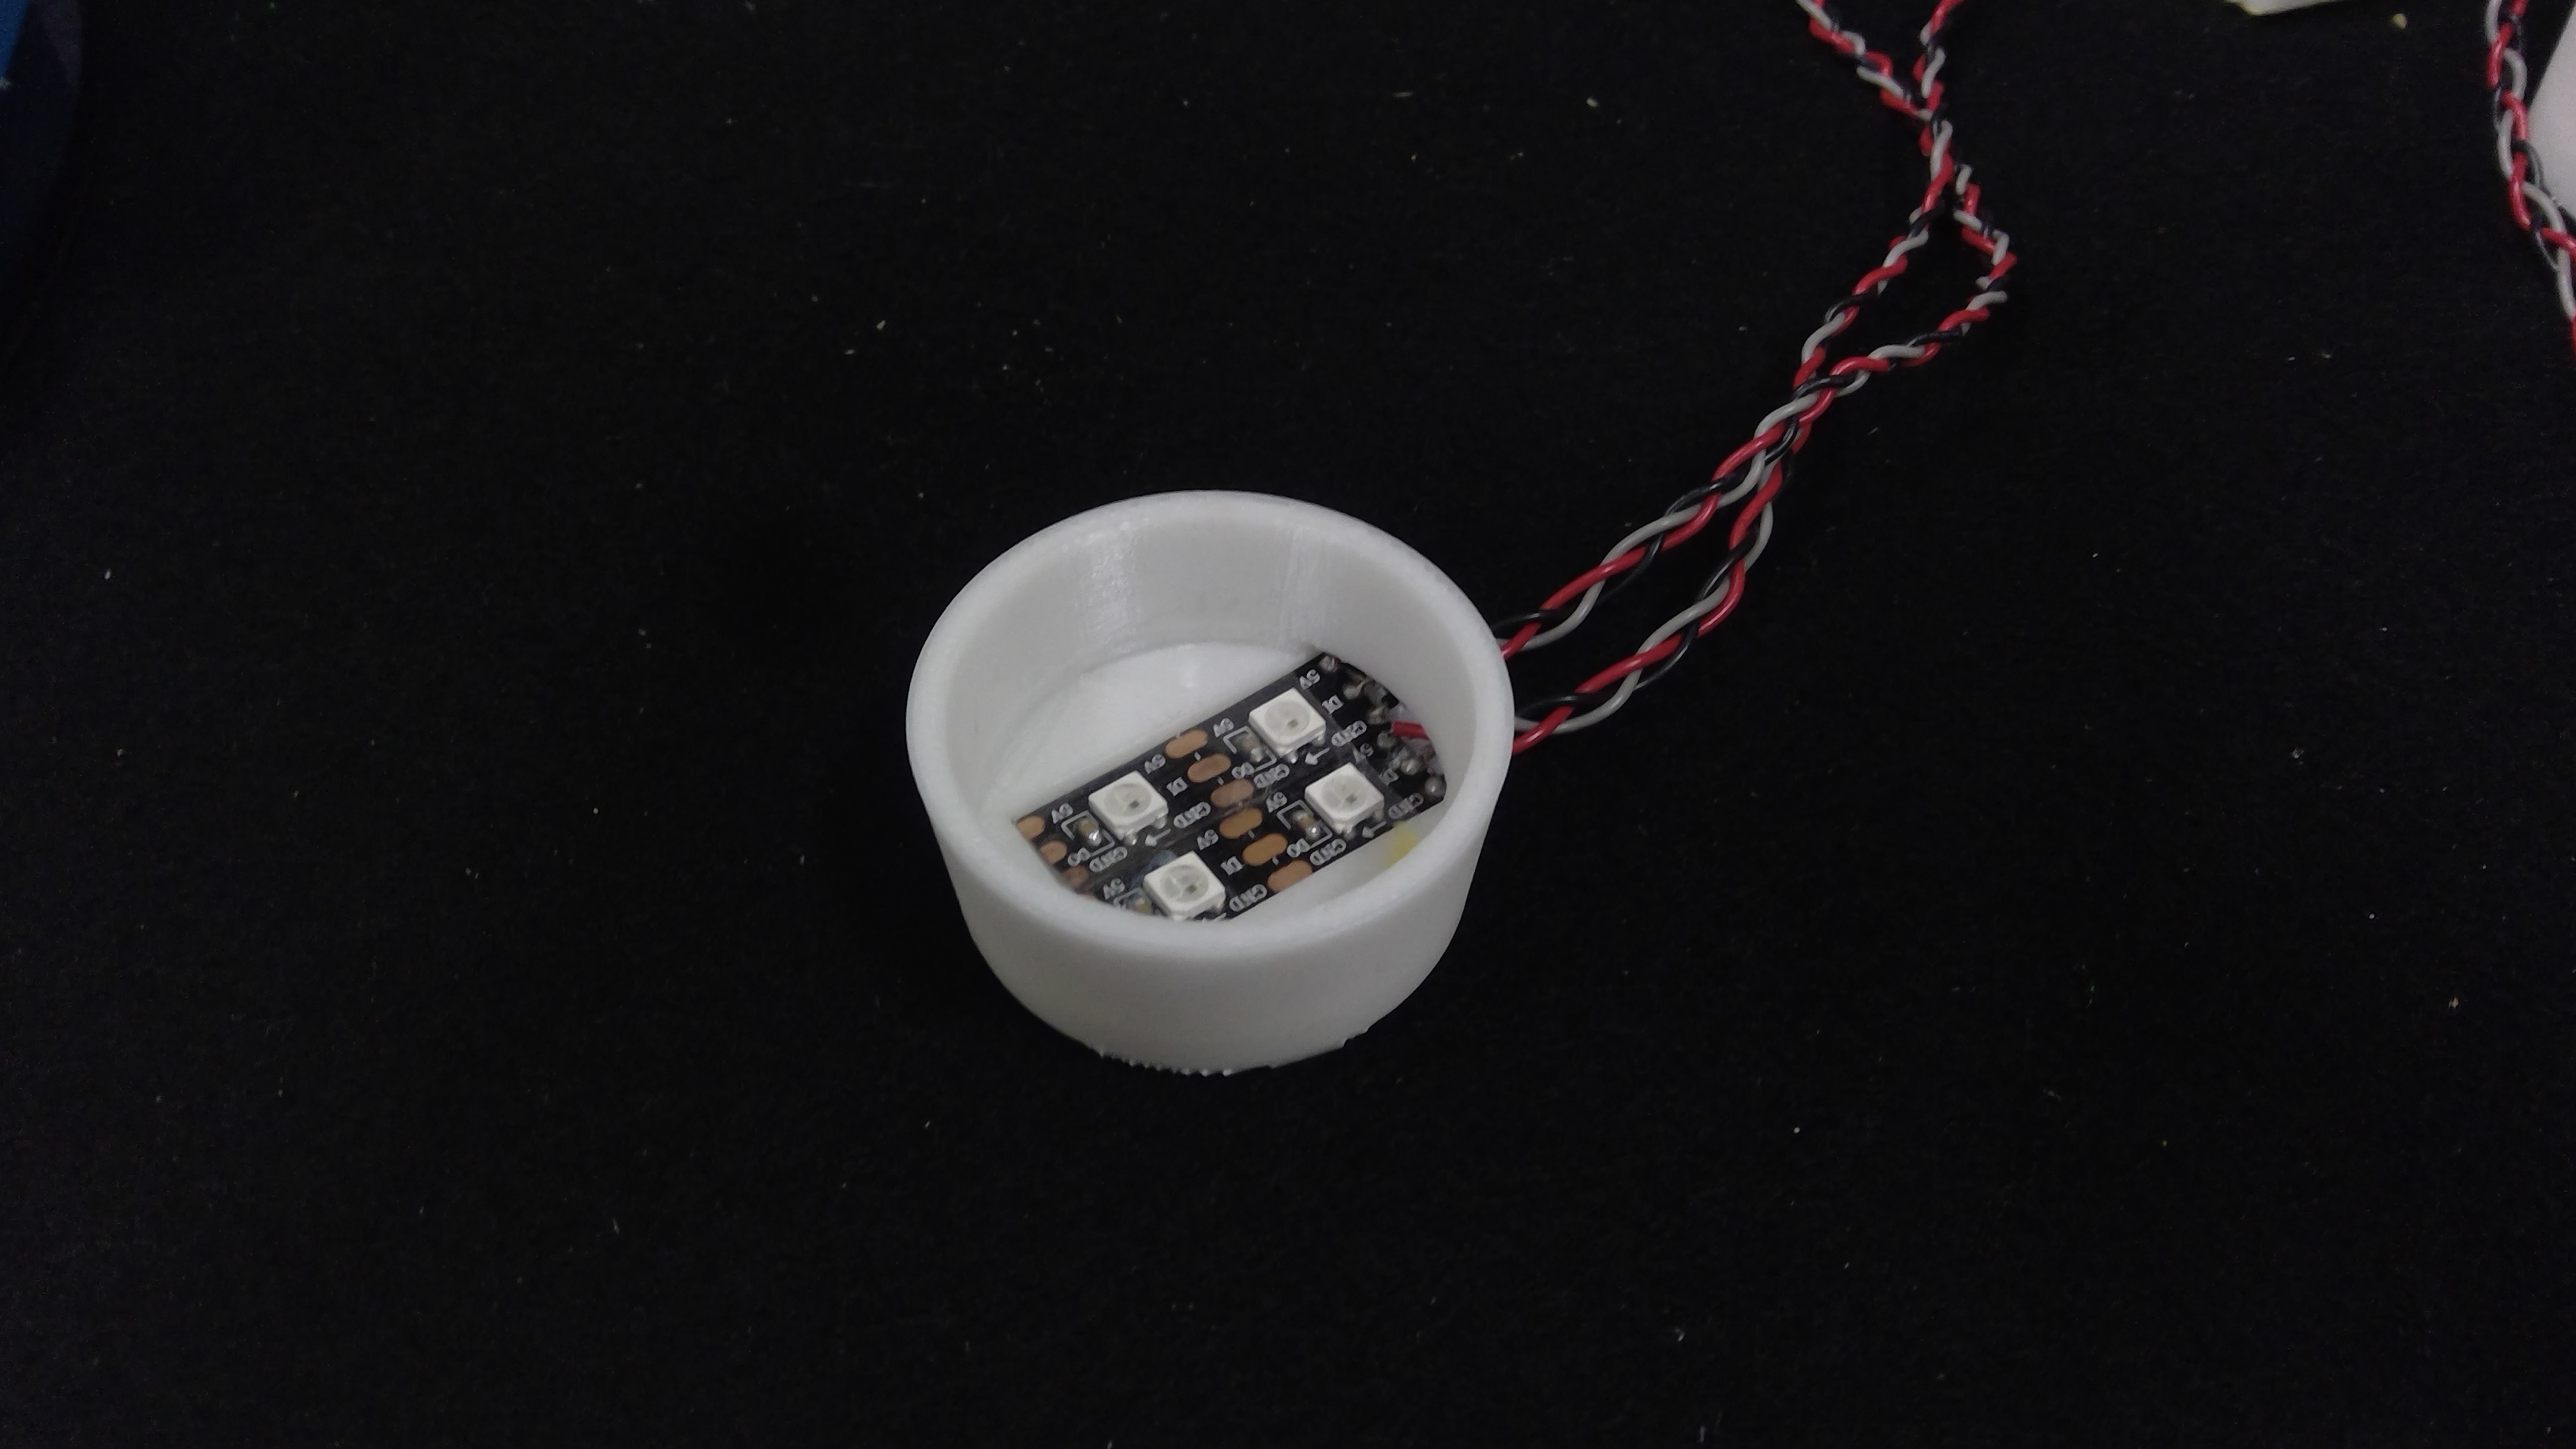
\includegraphics[scale = 0.075]{figs/coaster.jpg}
  \caption{LEDコースタ―}
  \label{coaster}
\end{figure}
\begin{figure}[t]
  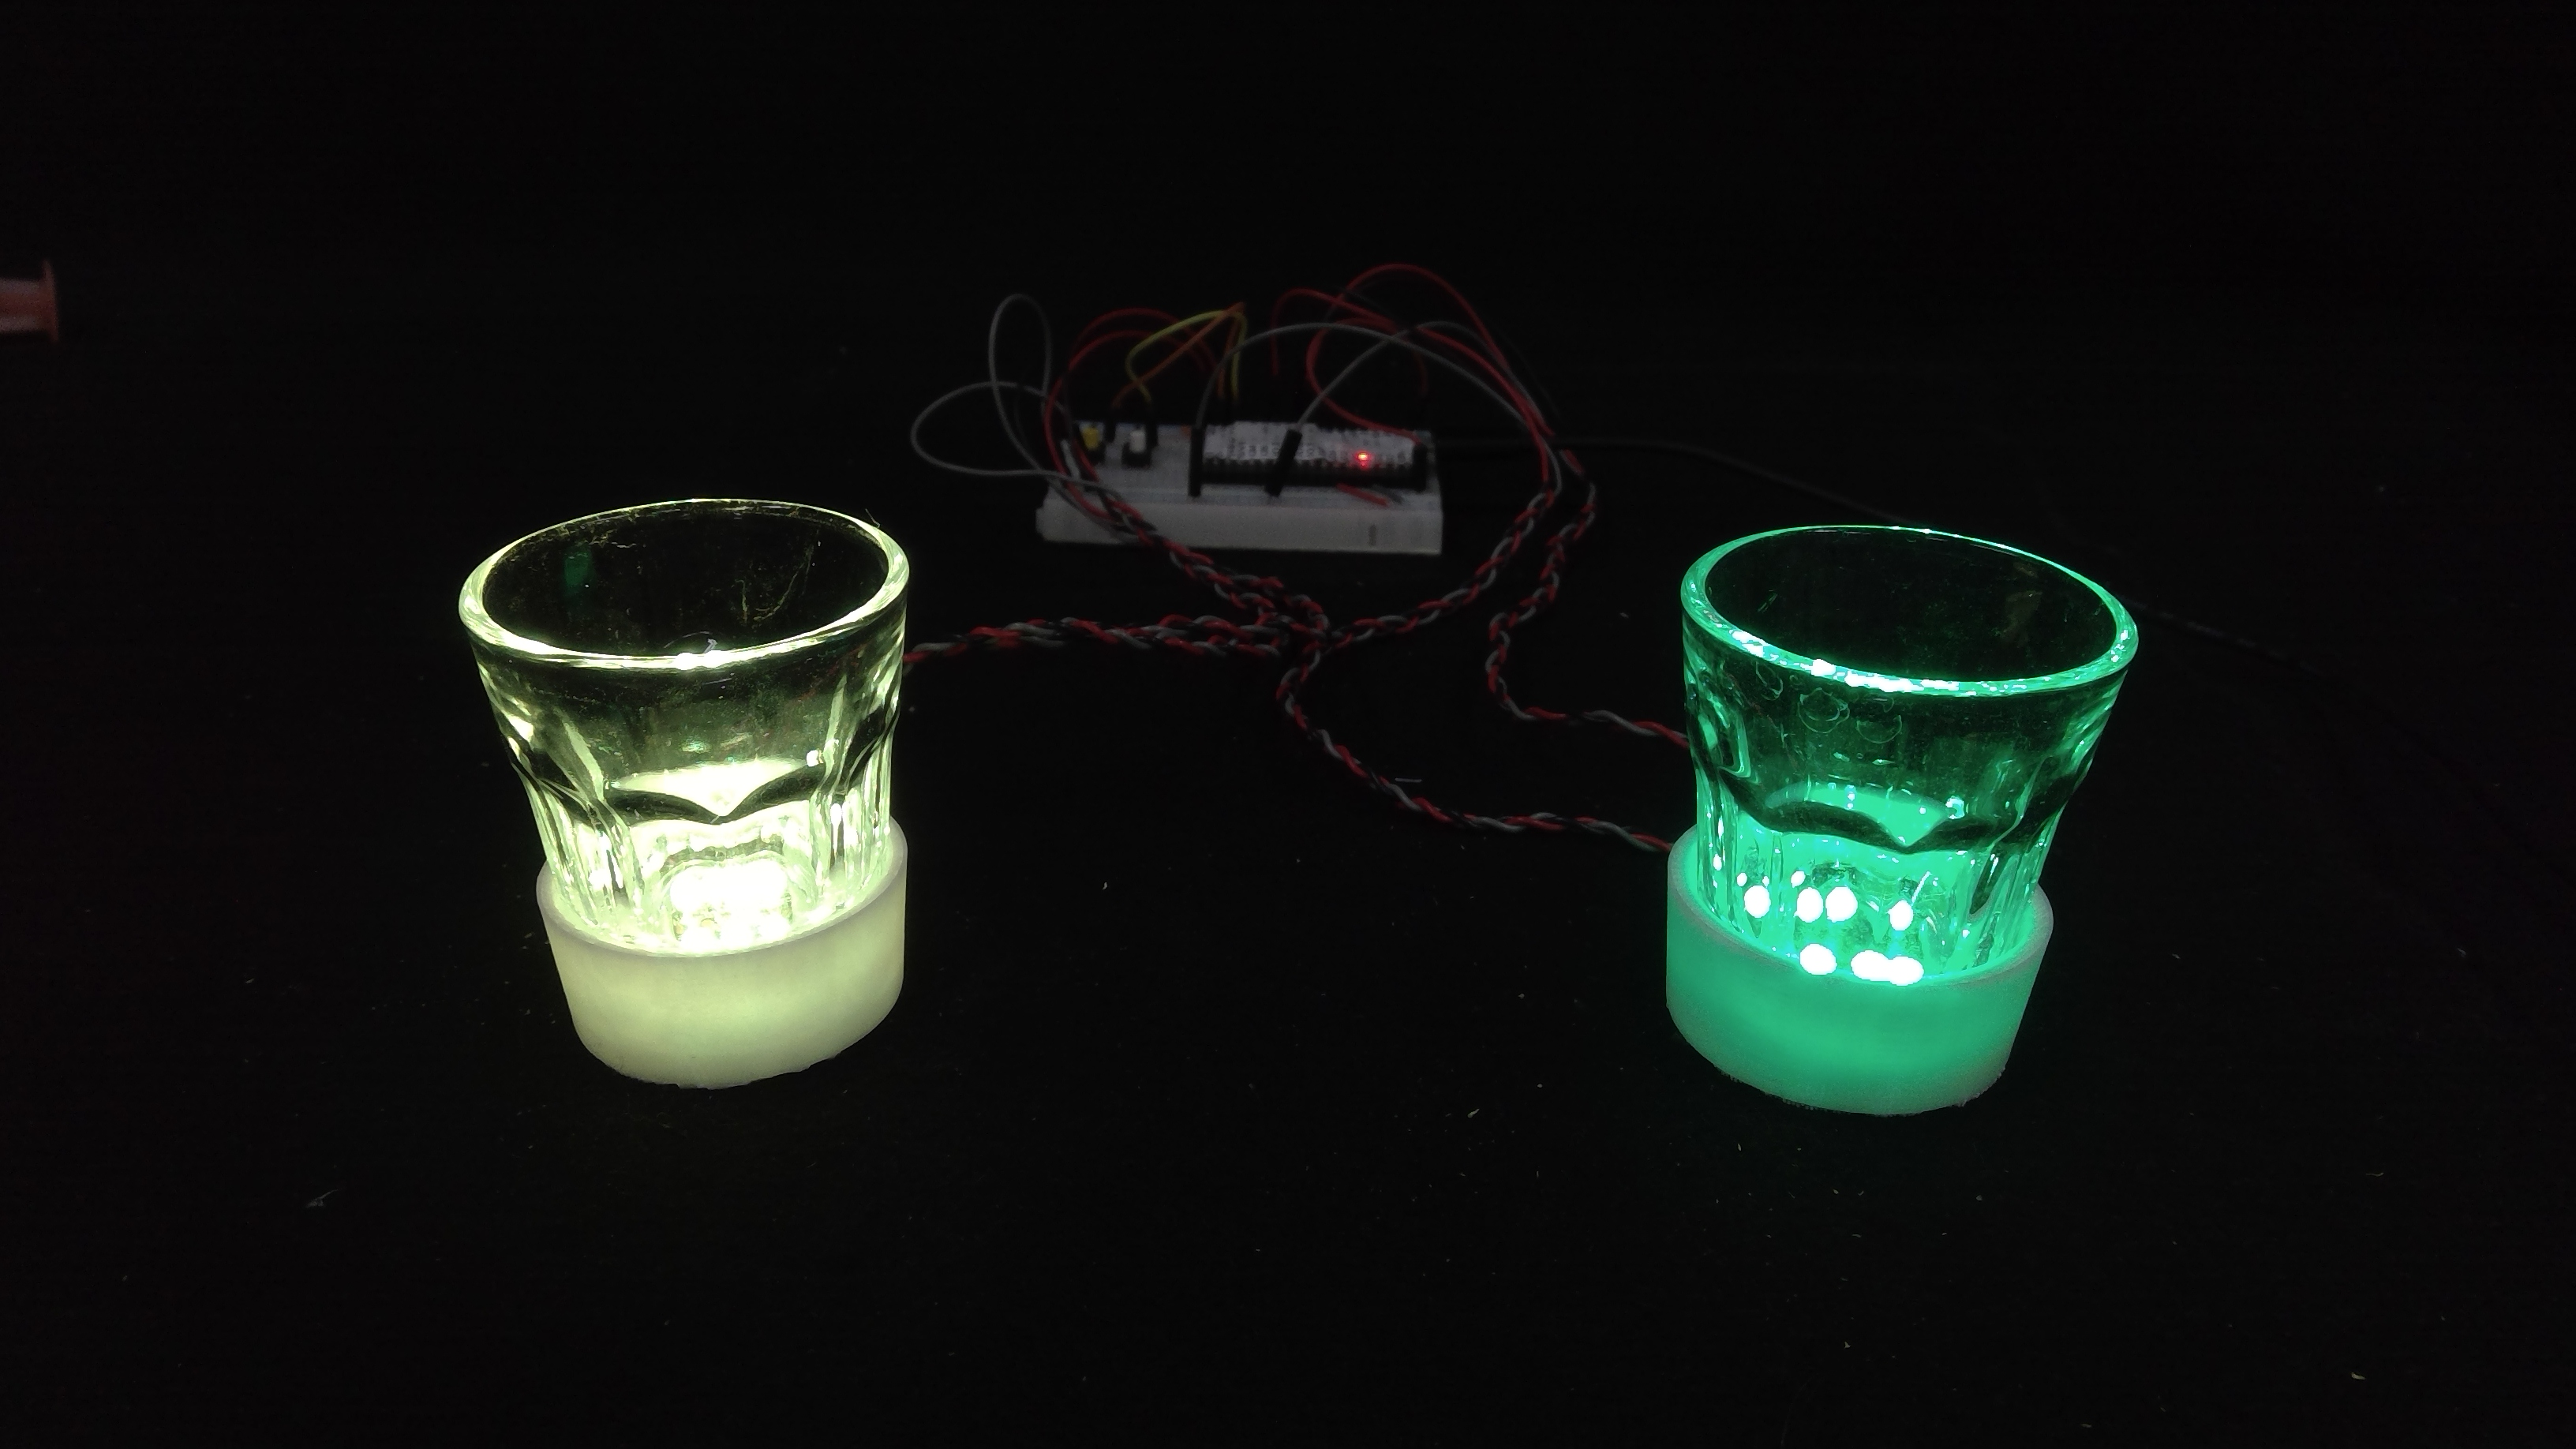
\includegraphics[scale = 0.075]{figs/gluss.jpg}
  \caption{LEDで照らされたショットグラス(黄色・緑色)}
  \label{gluss}
\end{figure}


かき氷におけるシロップの色の再現については,着色料の代わりとしてフルカラーのLEDを使用した.
LEDテープを透明なショットグラスの裏に設置するために図\ref{coaster}のようなコースターを作成した.
LEDの上面は透明なテープで覆うことで,ショットグラスから垂れる水滴が入らないようにしている.
このコースターを使用することで図\ref{gluss}のように,かき氷自体を照らすことが可能になり,また容器を持ち上げることができ,食べる瞬間まで色を感じることができる.
LEDの制御として,その場での切り替えをするためにタクトスイッチを用意し,それによって点灯または消灯の制御を行っている.
通常のかき氷では,削られた氷の上面にシロップの色がついているものだが,今回は色の印象強く与えることによる錯覚を重視し,かき氷全体に色を付けることとした.

%色がついているという印象を強く与えることを優先したために,この手法を採用することとした.
この手法を用いると,LEDの熱で氷が解けることが懸念されるため検証を行った.部屋の気温を22度で設定し,LEDコースターで照らされたかき氷は,4分以上はある程度の形を保ったままであった.そのため,実験の際には支障がないと判断した.

%\begin{figurfee}
%  \includegraphics[width = 0.32\columnwidth]{ice.jpg}
%  \includegraphics[width = 0.32\columnwidth]{ice2.jpg}
%  \includegraphics[width = 0.33\columnwidth]{ice3.jpg}
%  \caption{スプーン側のLED
%  (無色・黄色・白色)}
%  \label{ice}
%\end{figure}

LEDを使用する理由として,色の切り替えをスムーズに行えるという点が挙げられる.近年では見た目を変える手法としてはVRを使った手法がたくさん行われているが,可用性に欠けたり,食べ辛かったりする.そこでデバイスを渡すだけで簡単に行えることや現実的な視覚としての実験を行うことに意味があると考えた.また,関連研究にも挙げた「LED光源を用いて色を重畳した場合にも,着色料を用いて色を付けた際と同程度のクロスモダリティ効果があった」という実験結果を踏まえても,この手法は有意義であると考える.

色の選択として,使用する2種類の香りの印象の強い色を使用しショットグラスの容器を照らした.レモンの色を黄色,メロンの色は緑色とした.

\subsection{嗅覚情報提示}
香りを嗅がせる方法として,図\ref{all}の嗅覚情報提示装置を製作した.
香りを送るための仕組みを含んだボディやケースを3Dプリンタで作成している.
全体の流れの構成を図\ref{flow}に示す.エアポンプから配送された風はチューブを通り,制御されたエアー分岐管を通ることで3つの経路に分かれる.2つの経路では,香りを含ませた脱脂綿を仕込んだ香り瓶の中を経由して香料を付与した風となり,残りの一つは何も含まない風となる.この3つをまとめたものがスプーンデバイスに組み込まれており,スプーンを口に運んだ際に,鼻に香りを付与した風が当たるものとなっている.


\begin{figure}[t]
  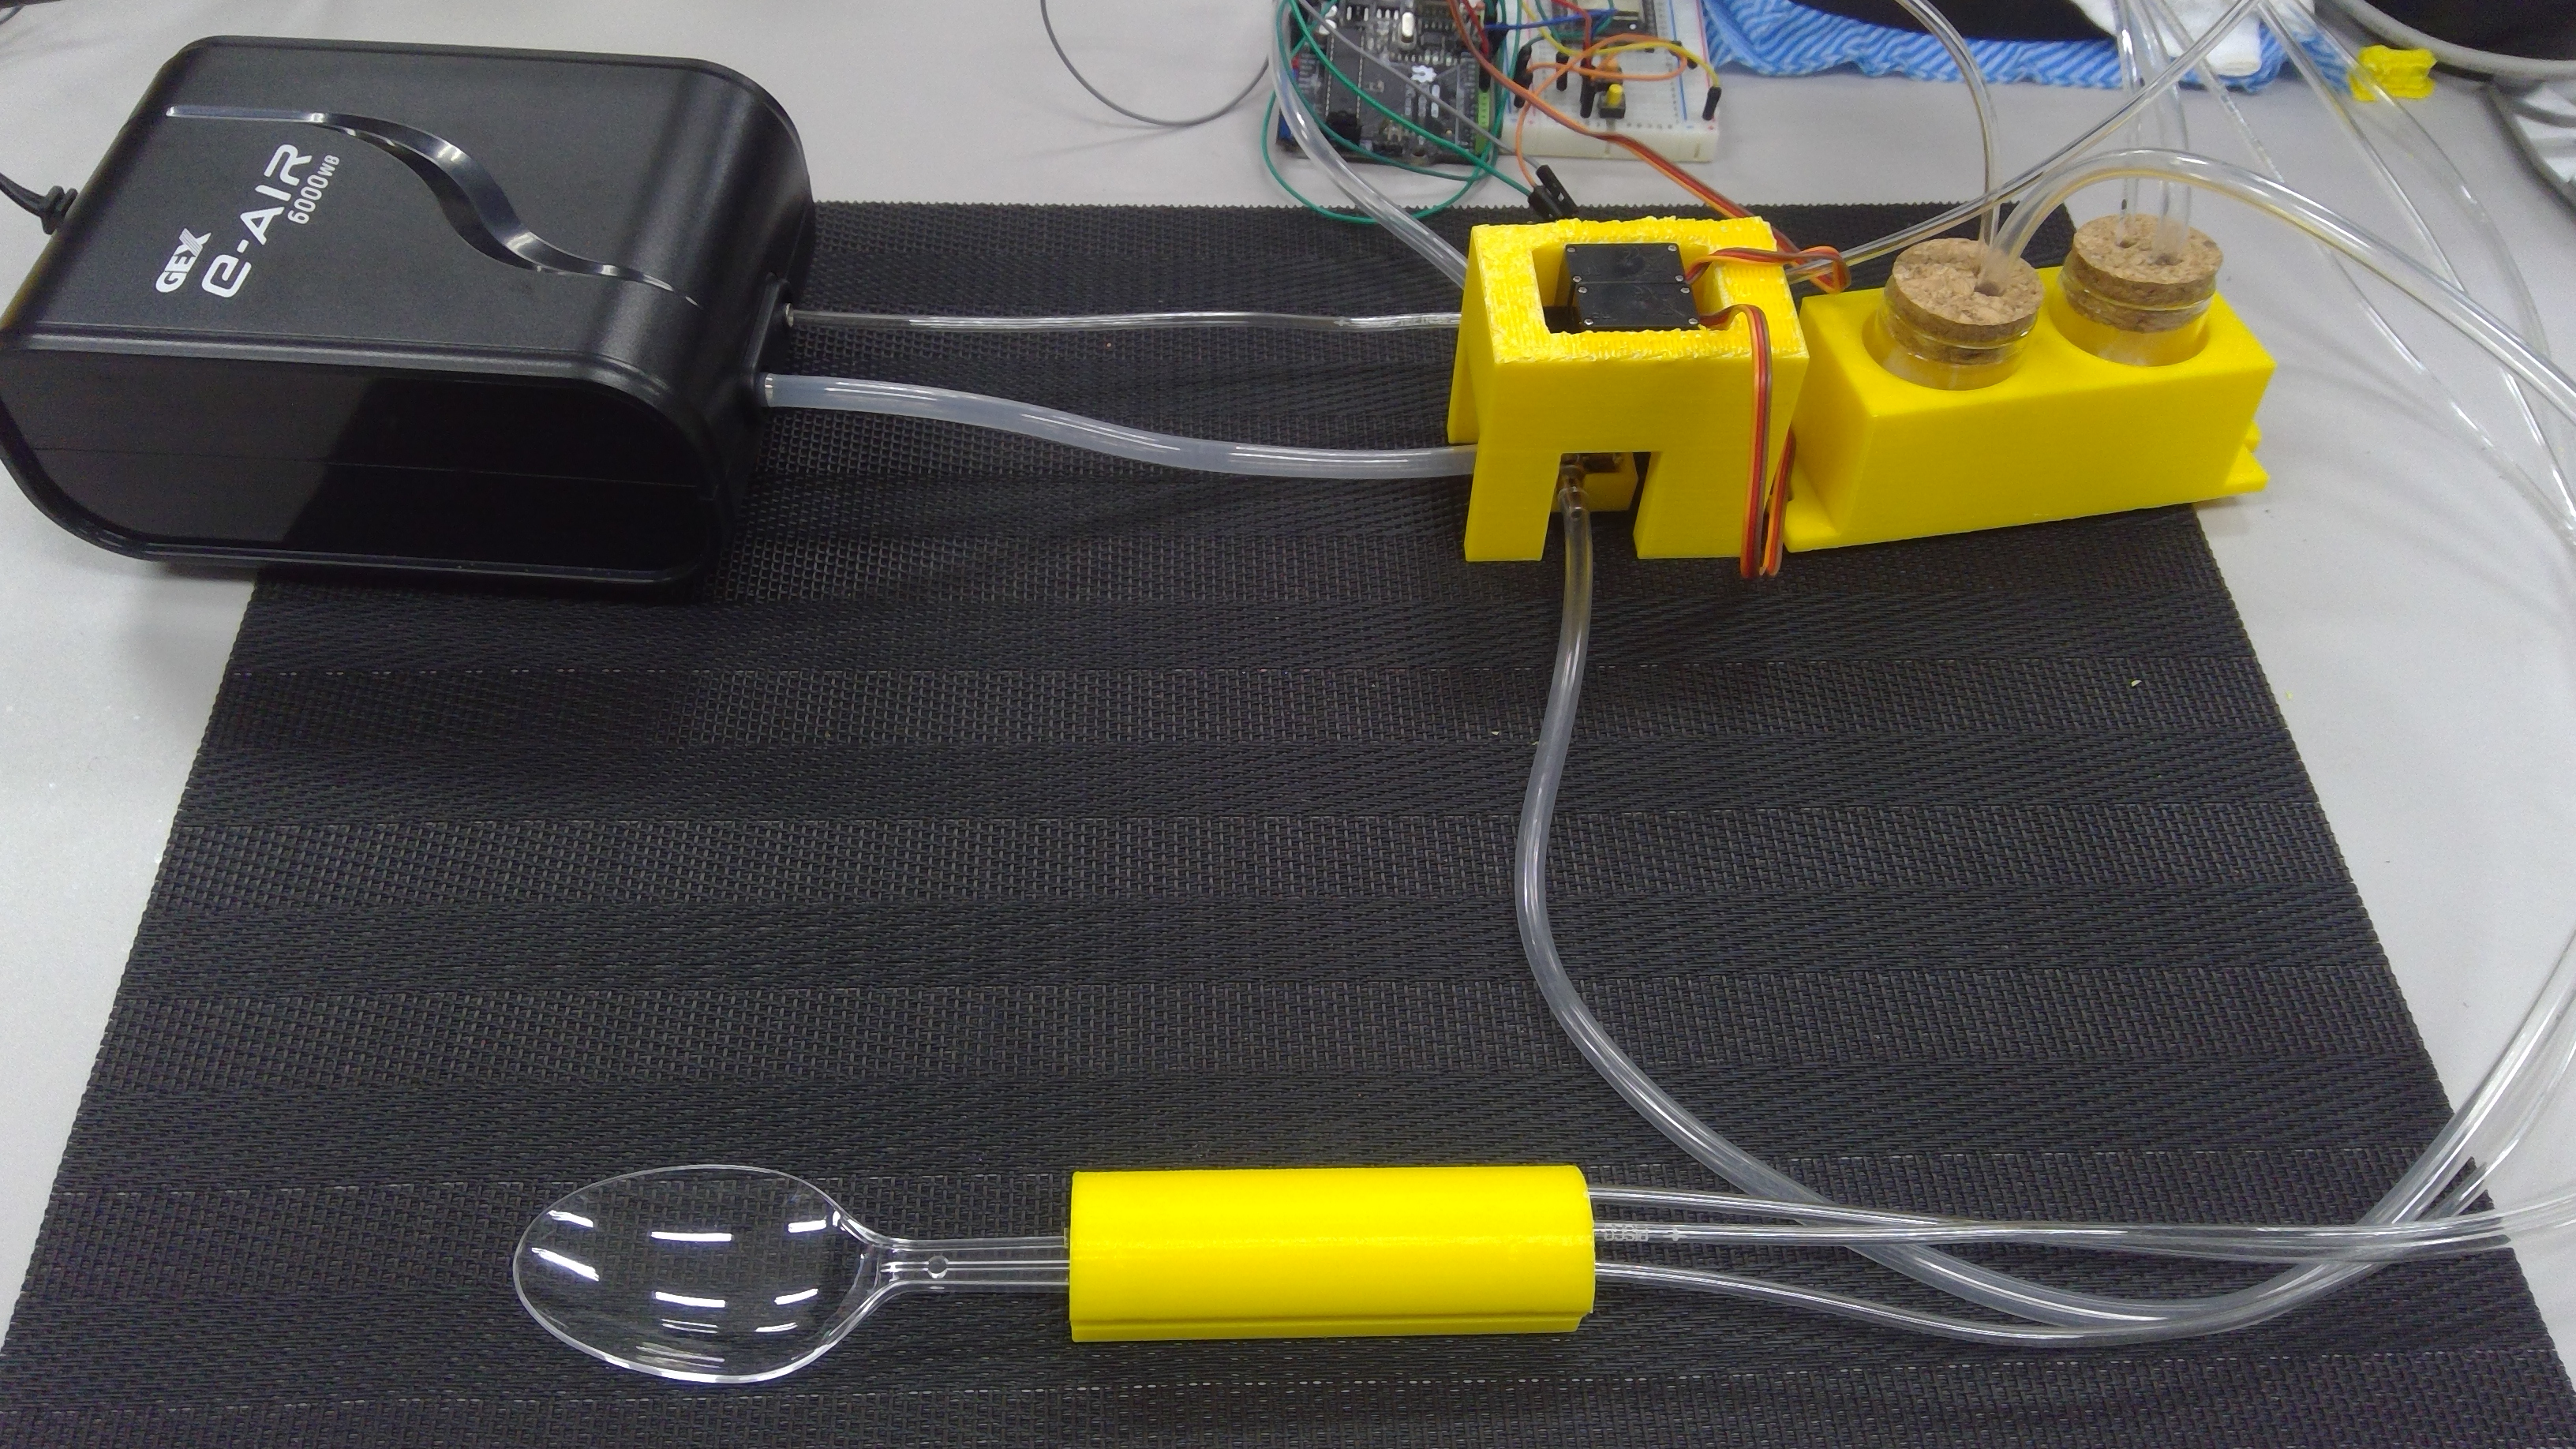
\includegraphics[width = 1.0\columnwidth]{all.jpg}
  \caption{嗅覚情報提示装置の全景}
  \label{all}
\end{figure}

\begin{figure}[t]
  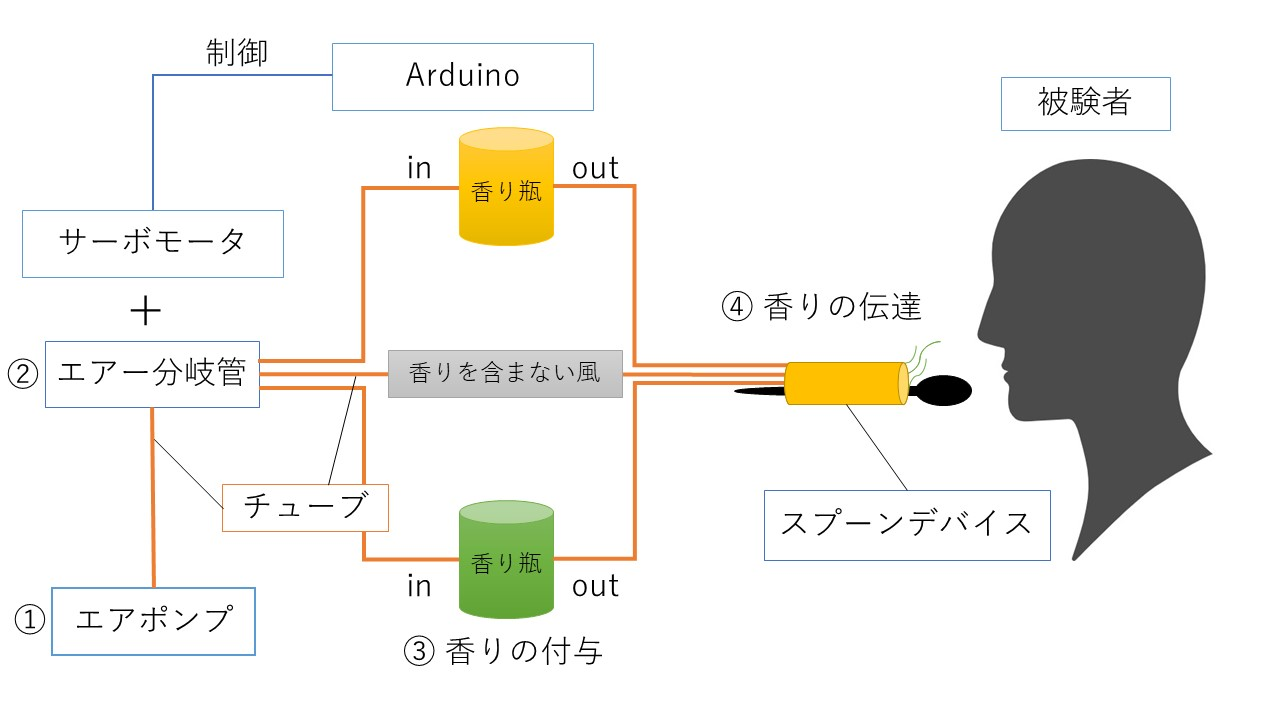
\includegraphics[width = 1.0\columnwidth]{flow.jpg}
  \caption{香り配送の流れ}
  \label{flow}
\end{figure}


\subsubsection{香料}
かき氷のシロップに含まれている香料の代わりとして,レモン・メロンの2種類の香りを外部刺激として使用する.

レモン・メロンは共に既存のシロップの味として存在しており,出店にもあるベーシックな味である.レモンは以前の研究から,有効性が確かめられており,デバイスが変わっても有効性を調査するために選んだ
.メロンの香りは新たな香りの検証として,甘味を感じやすい香りという点からも味の違いに差が出るのではないかと仮説を立て,選択した.

香りを感じさせる方法は,レモンはアロマオイル(天然植物精油)を使用し,メロンは市販の食品添加物から,それぞれ液体となっている香料を脱脂綿に染み込ませ,その香りを嗅がせることとした.この実験においてはレモンの味の再現としてレモンの香りではなくライムの香りを使用している.以前の研究の予備実験において,10人に対してどちらのほうがレモン味のかき氷の香りに近いかを尋ねたところ,ほとんどがライムの香りを選択している.ライムの香りのほうがレモン味のかき氷の風味に似ているという点から、今回もライムの香りを使用している.

\subsubsection{スプーンデバイス}
図\ref{device}に示したスプーンデバイスはスプーンとして持つ際に抵抗が出ないように作成している.
\begin{figure}[t]
  %\includegraphics[width = 0.47\columnwidth]{front2.jpg}
  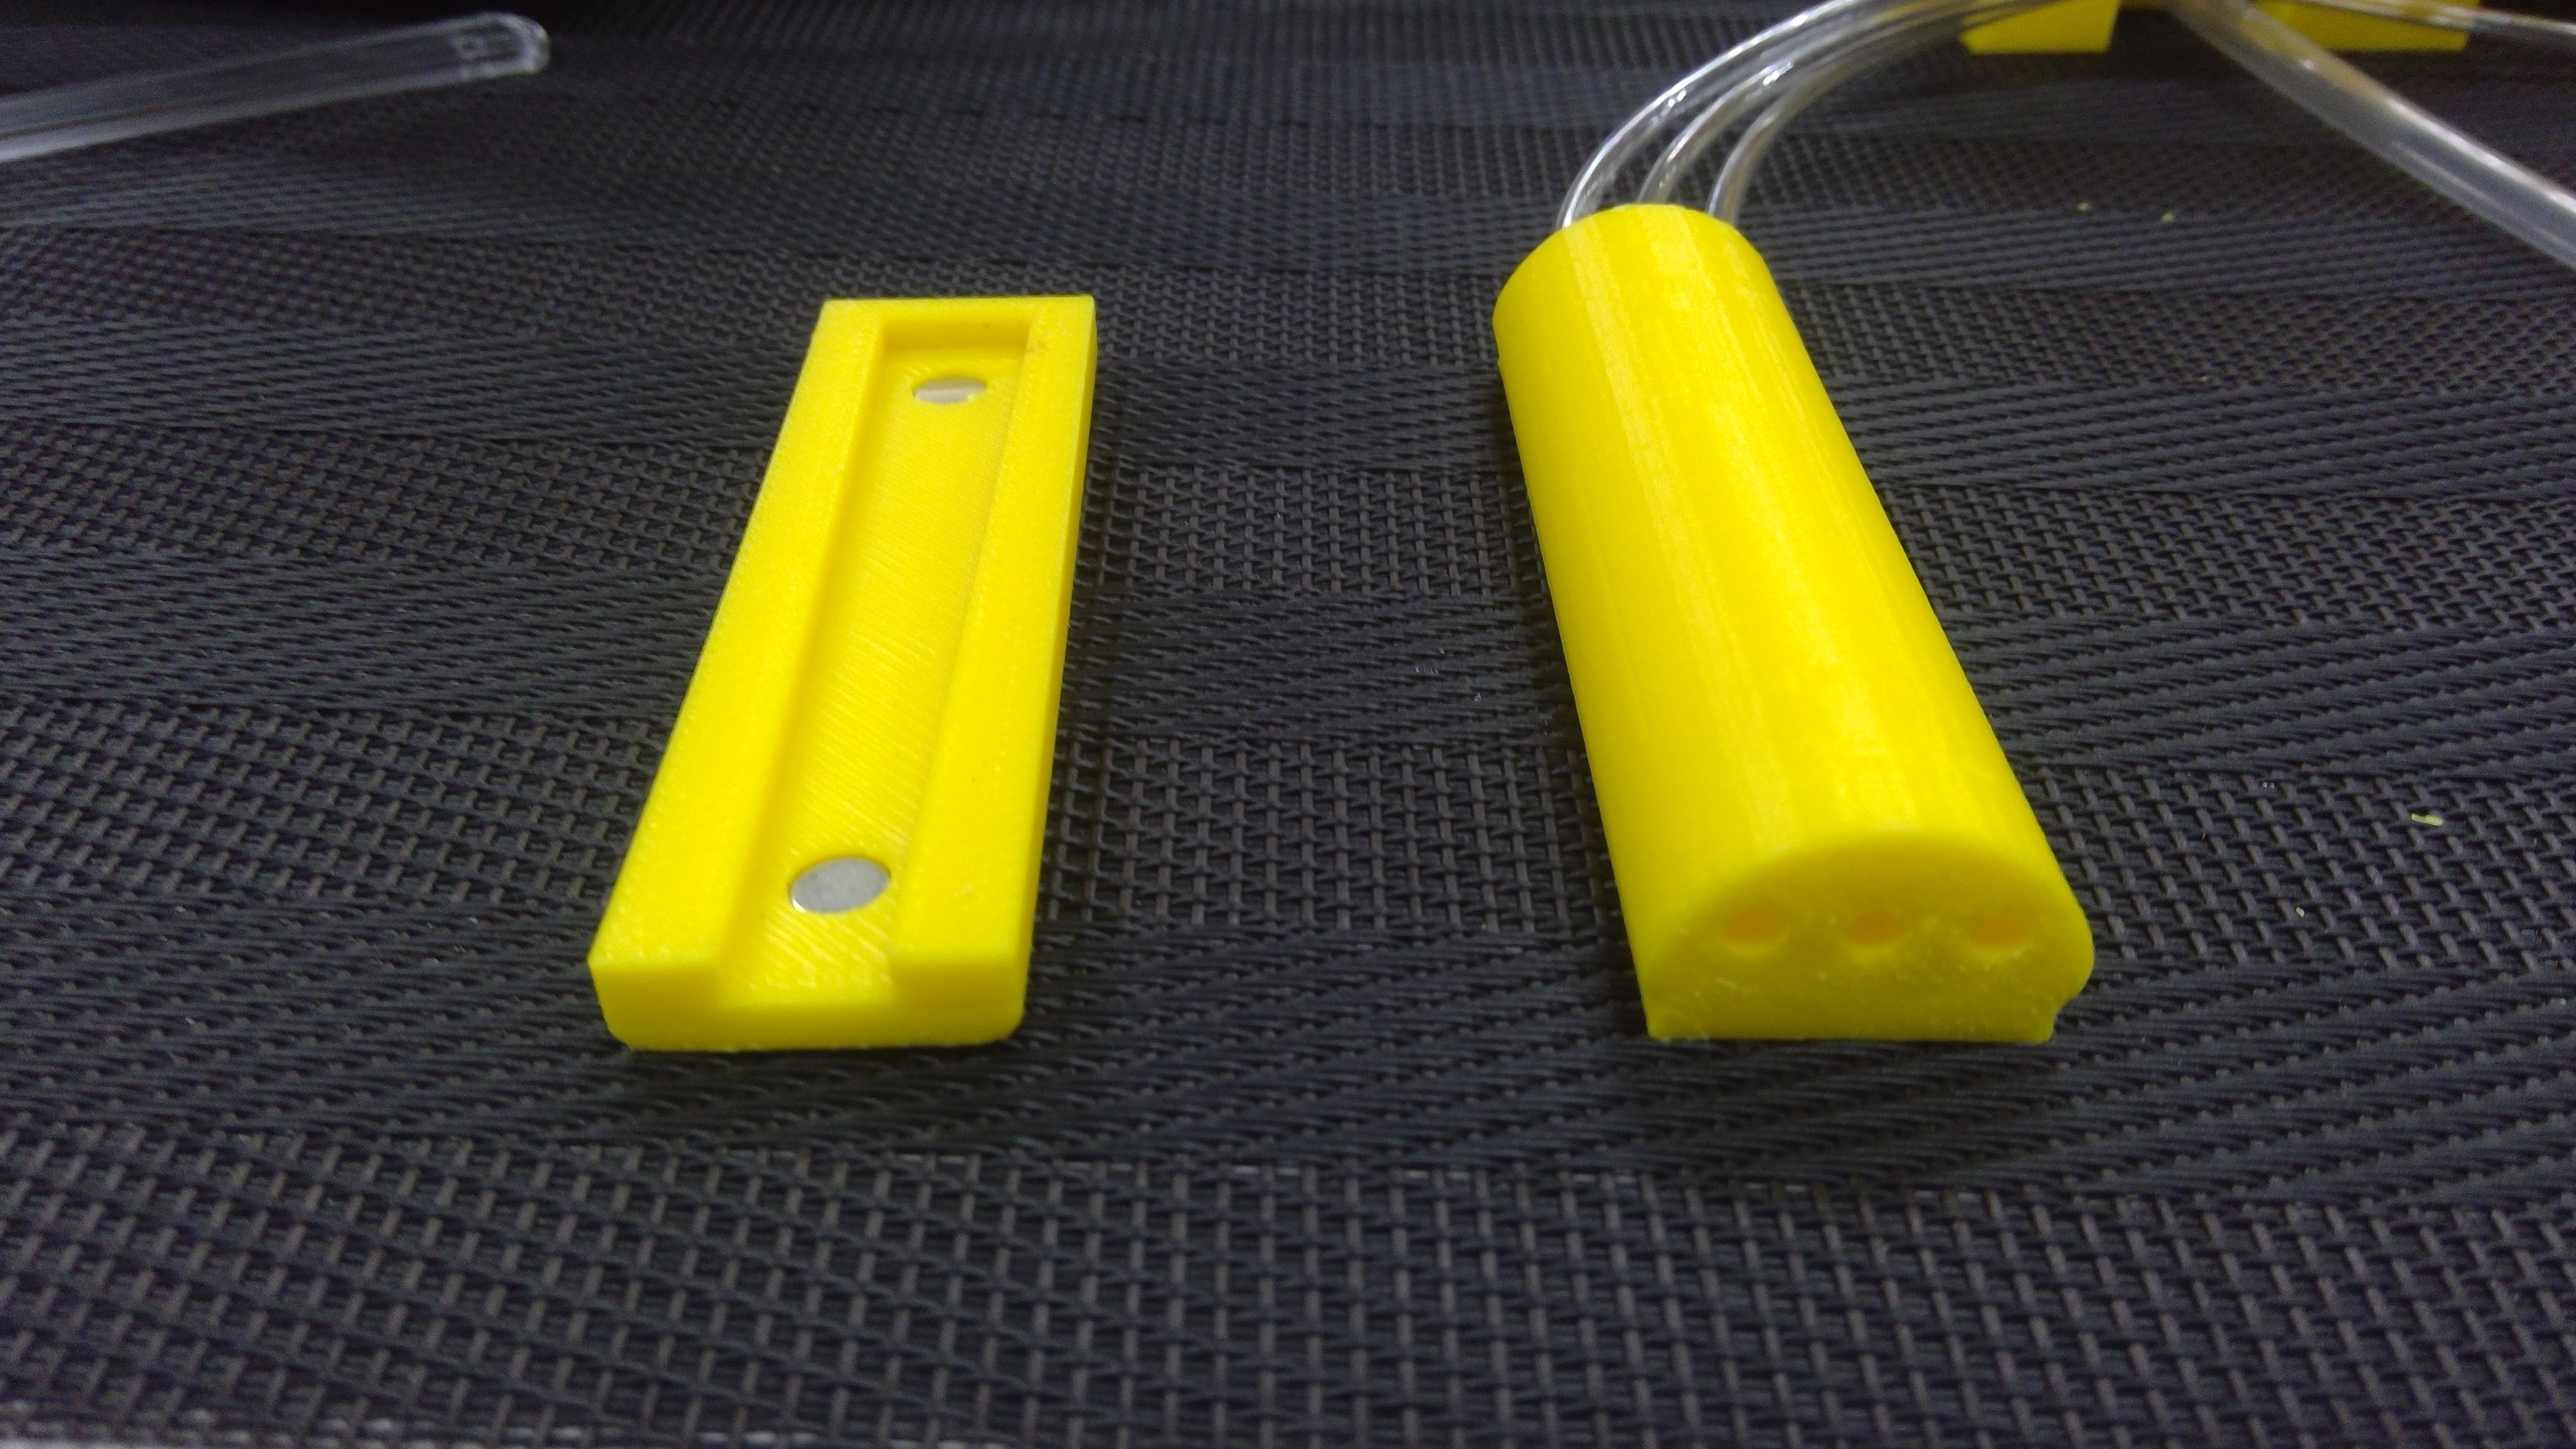
\includegraphics[width = 1.0\columnwidth]{supunpart.jpg}
  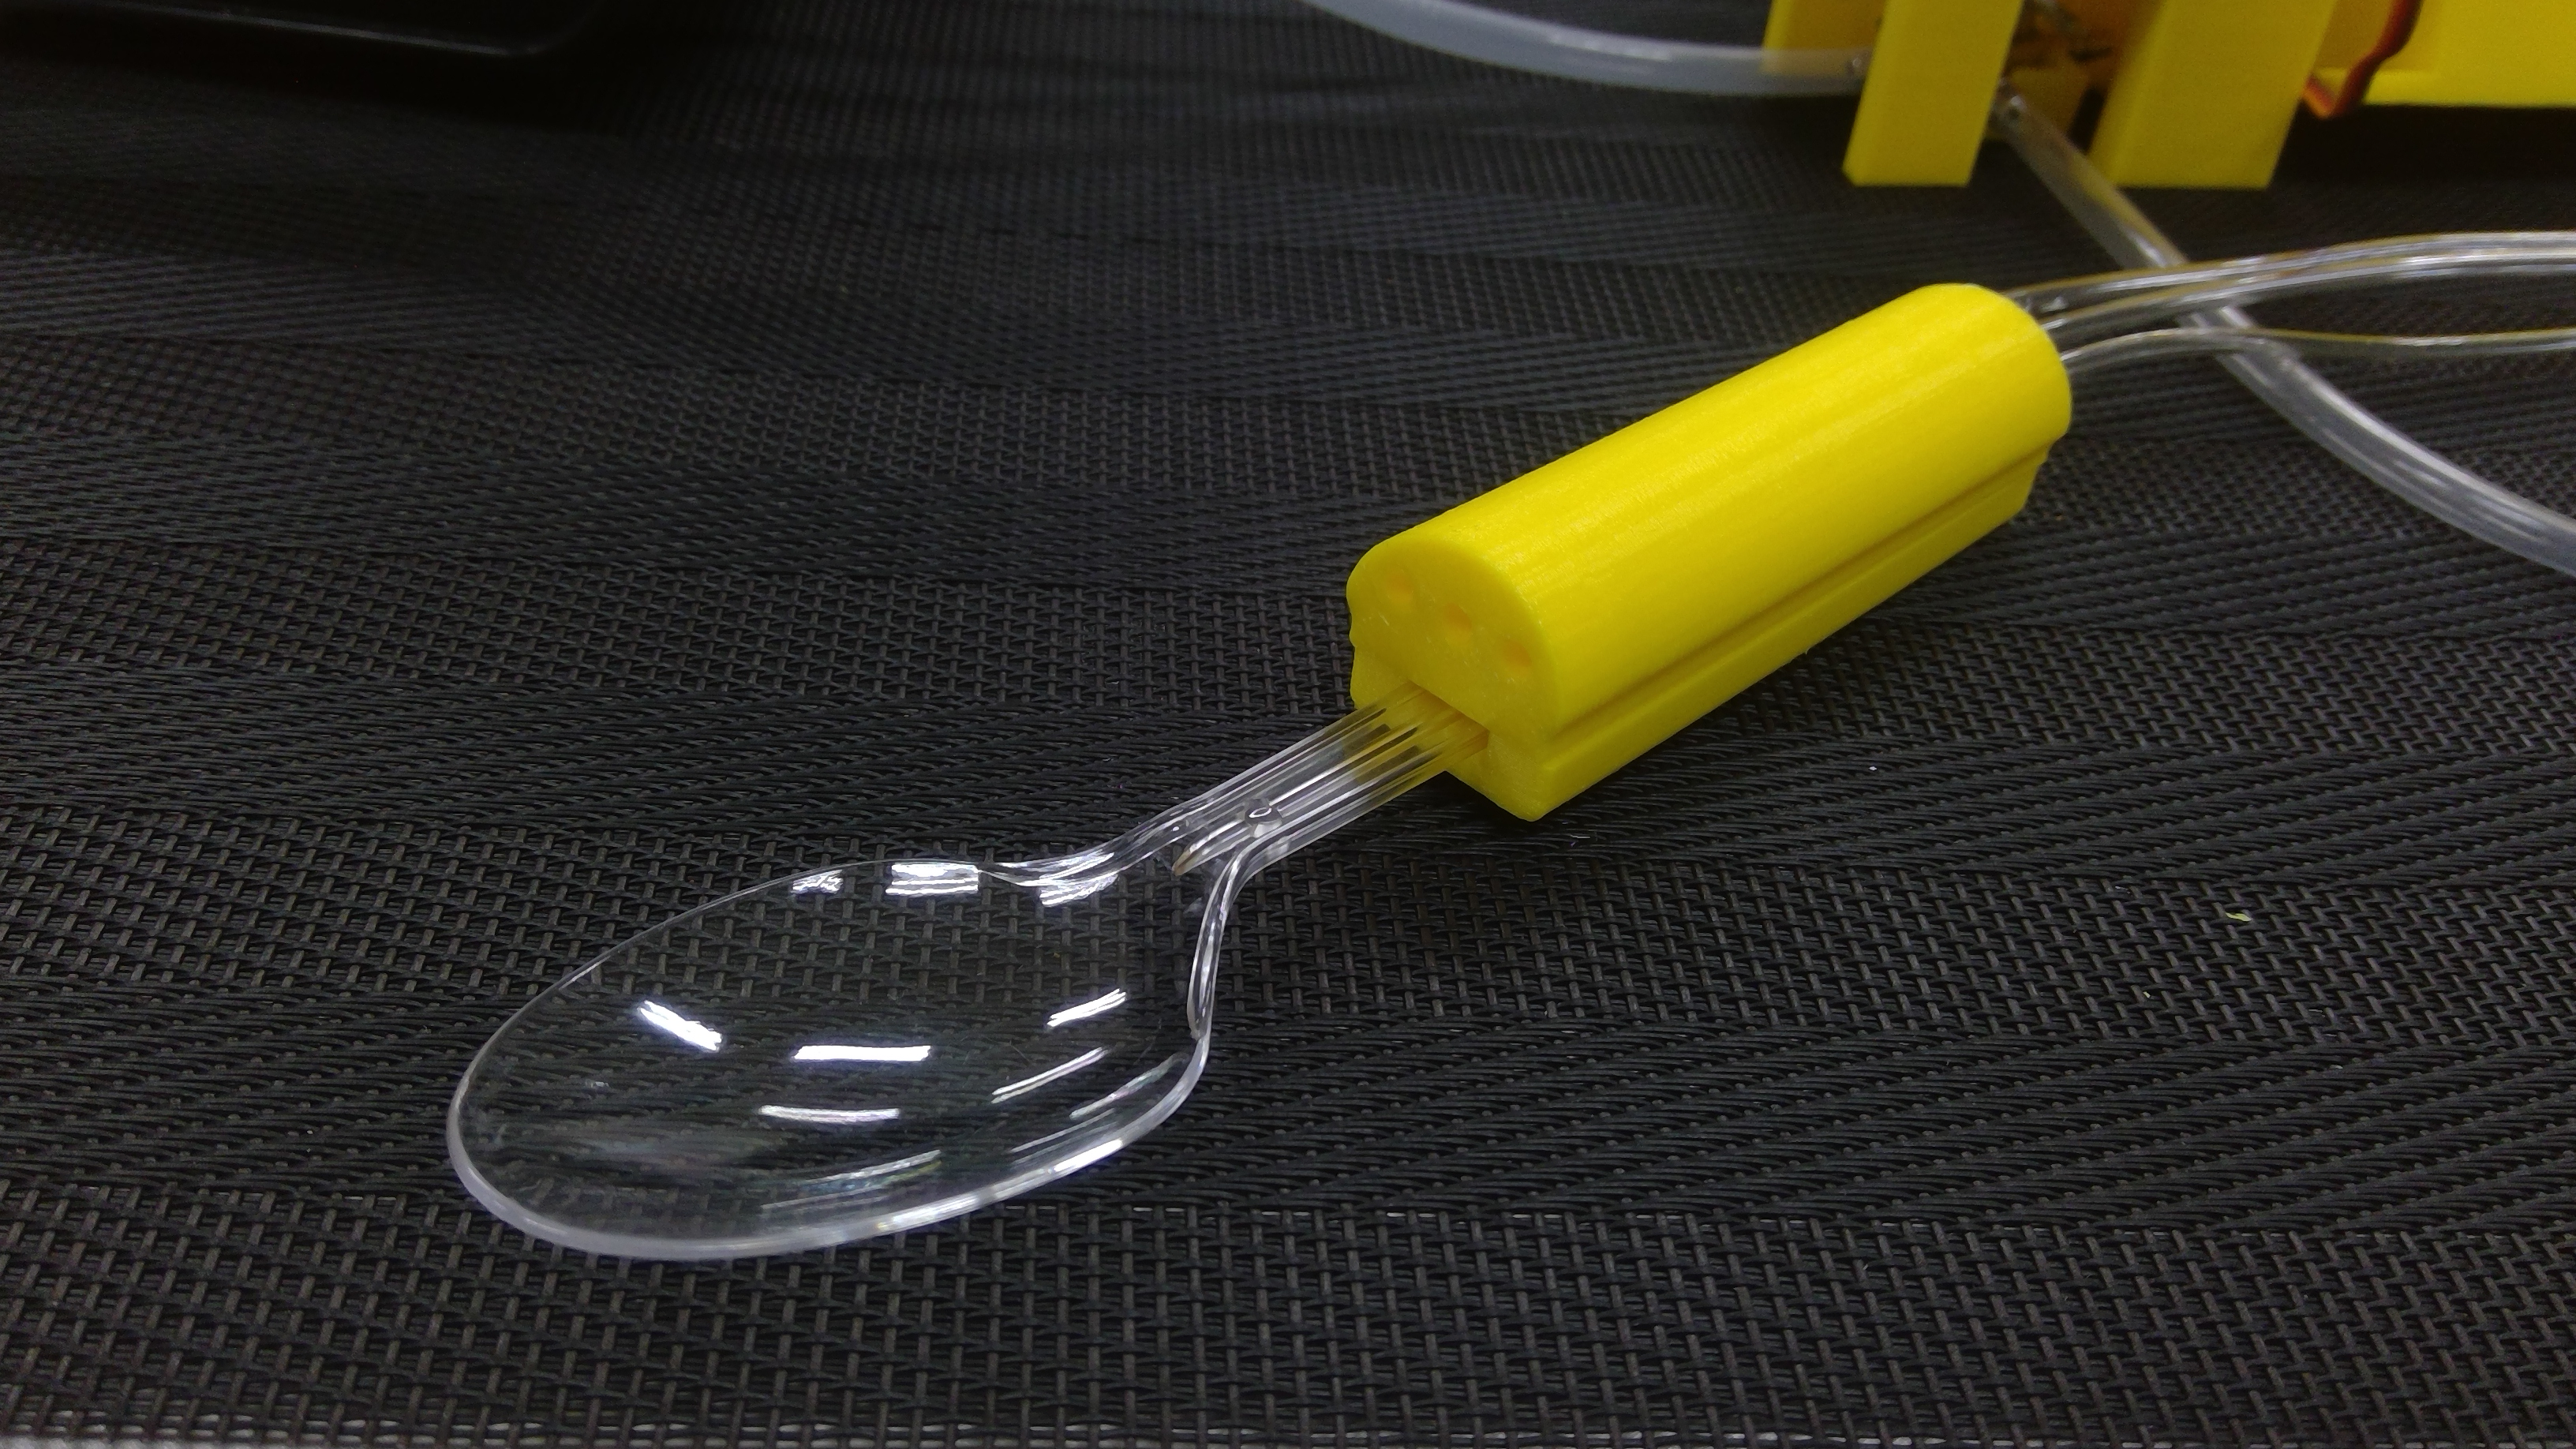
\includegraphics[width = 1.0\columnwidth]{supunbody.jpg}
  \caption{スプーンデバイス
  (上部・下部・全体)}
  \label{device}
\end{figure}
以前の研究では,ファンの大きさに合わせた四角柱の形をしており,持つことが非常に困難となっていた.そのために,手にフィットするちょうどよい大きさで作成している.
ボディは二つに分解することができ,これはスプーンの取り外しが簡単にすることができるようにするためである.上部のボディには香りを送るためにエアチューブを3本通している.そのうちの二つからは香りを含んだ風が流れ,残りは香りを含まない風を流す.下部のボディにはスプーンのサイズに合わせた溝を作っており,そこにスプーンをはめ込むことができる.かき氷を食べる食器は市販の透明なプラスチックスプーンを使用する.衛生面も考慮したうえで使い捨てのスプーンであることを重視し,ショットグラスのLEDの色が見えるように透明なスプーンを選択した.上部と下部のそれぞれボディに磁石を仕込むことで,二つのボディはくっつき安定する.この二つを組み合わせたボディをスプーンに取り付けることで口元にスプーンを運んだ時に,香りを含んだ風が鼻に当たる仕組みとなっている.




\subsubsection{香りの配送装置}
香りを配送する手段として,エアポンプによる風の配送で最終的にユーザーの鼻へと香りを届けている.風はゴムチューブを介して送られており,三又のエアー分岐管を経由することで,3つの経路に分けられる.分岐管には風の流れを制御するためにエアコックがついており,これにサーボモータを用いることで動きを制御する.図\ref{servo}のように,エアコックの上にサーボモータを設置し,二つを固定する.これによりArduinoで制御したサーボモータの動きと連動することでエアコックの開け閉めを可能とする.サーボモータの動きはタクトスイッチにより0度から90度の動きを指示し,これを香りを含ませる2つのチューブに対して実行する.
\begin{figure}[t]
  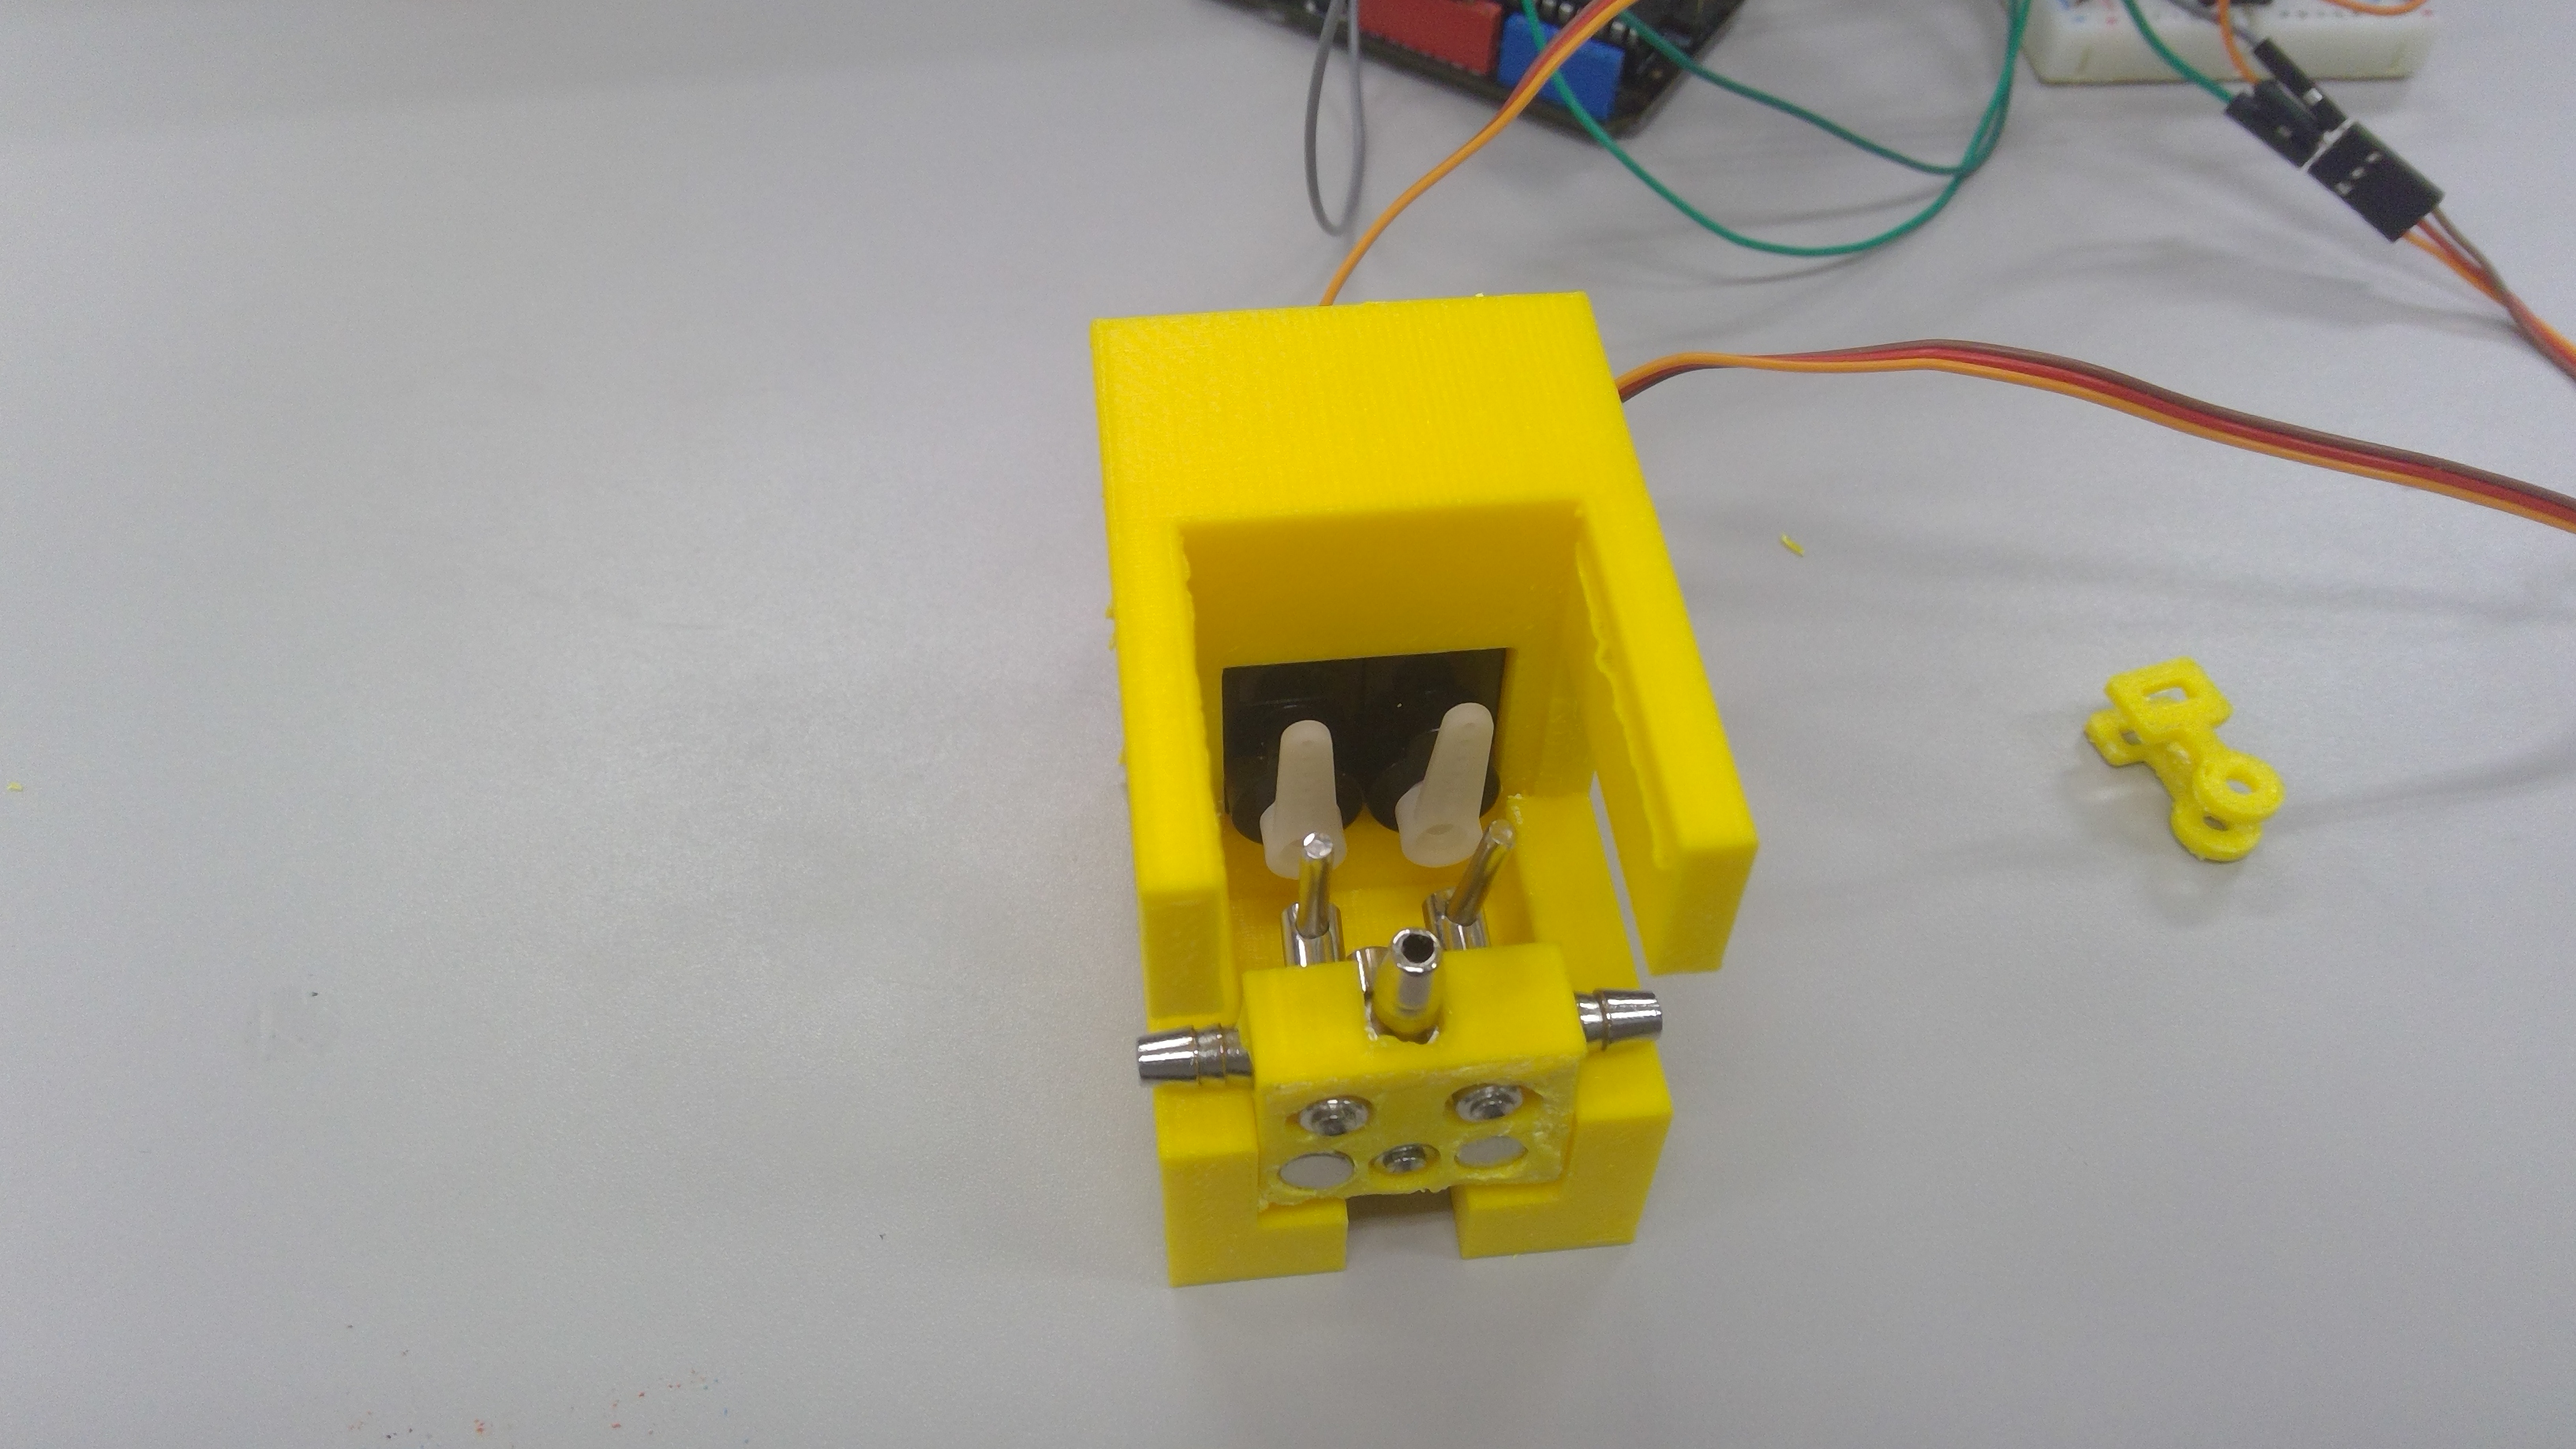
\includegraphics[width = 1.0\columnwidth]{servobox.jpg}
  \caption{サーボケースとエアー分岐管}
  \label{servo}
\end{figure}
この制御した風が流れる2つのチューブはそのまま図\ref{flavor}の香り瓶を経由することで香りを含ませることができる.前節で述べたように,今回はレモンとメロンの香りを用意しており,香り瓶の中にはこの二つの香りが仕込まれている.香り瓶の中には,香料を気化させやすくするために脱脂綿を入れる.香りを付与した風がそのままチューブを通じてスプーンデバイスへとつながる.残り1つのチューブでは何も含まない風を流し,制御せずにスプーンデバイスから流し続ける.これは香りを含んだ風を届ける際の補助となる風であり,配送していない際のスプーン周辺の換気のための風でもある.


\begin{figure}[t]
  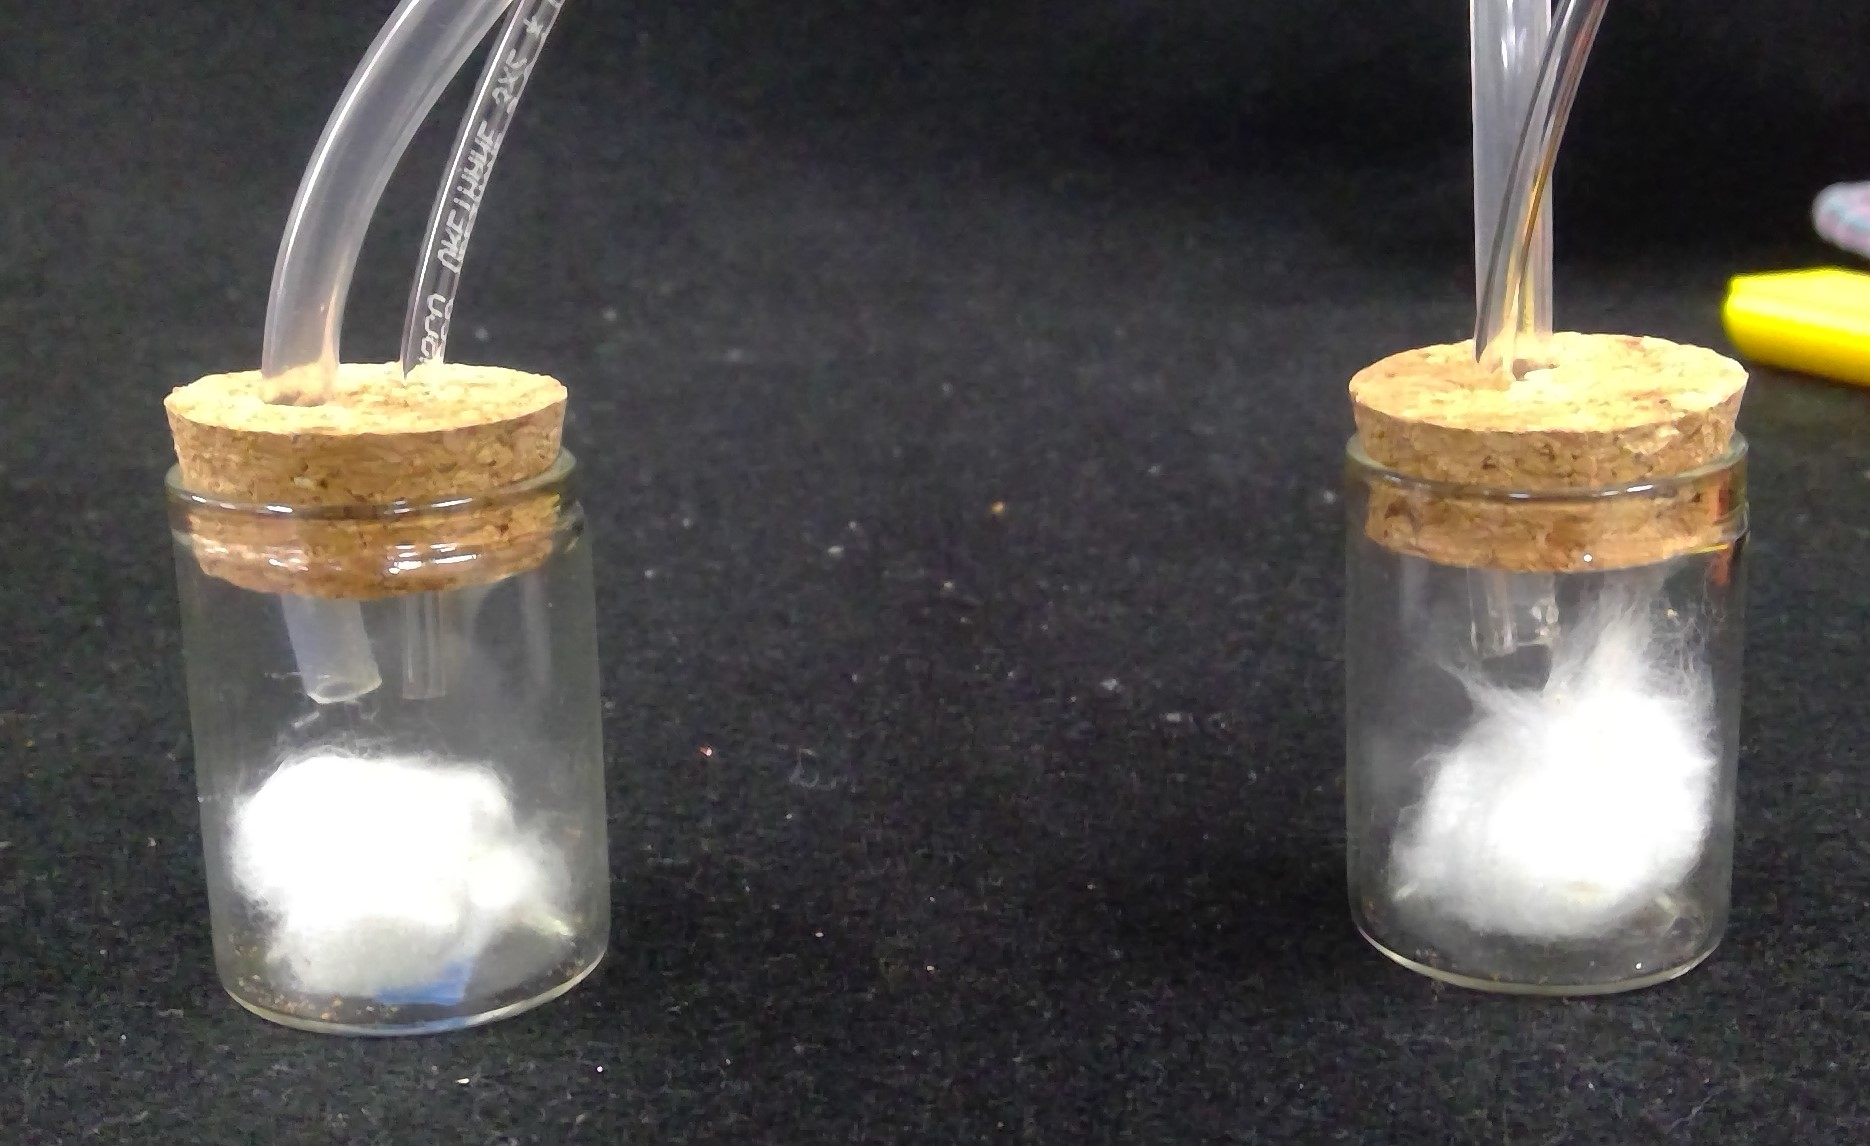
\includegraphics[width = 0.49\columnwidth]{flavorbin.jpg}
  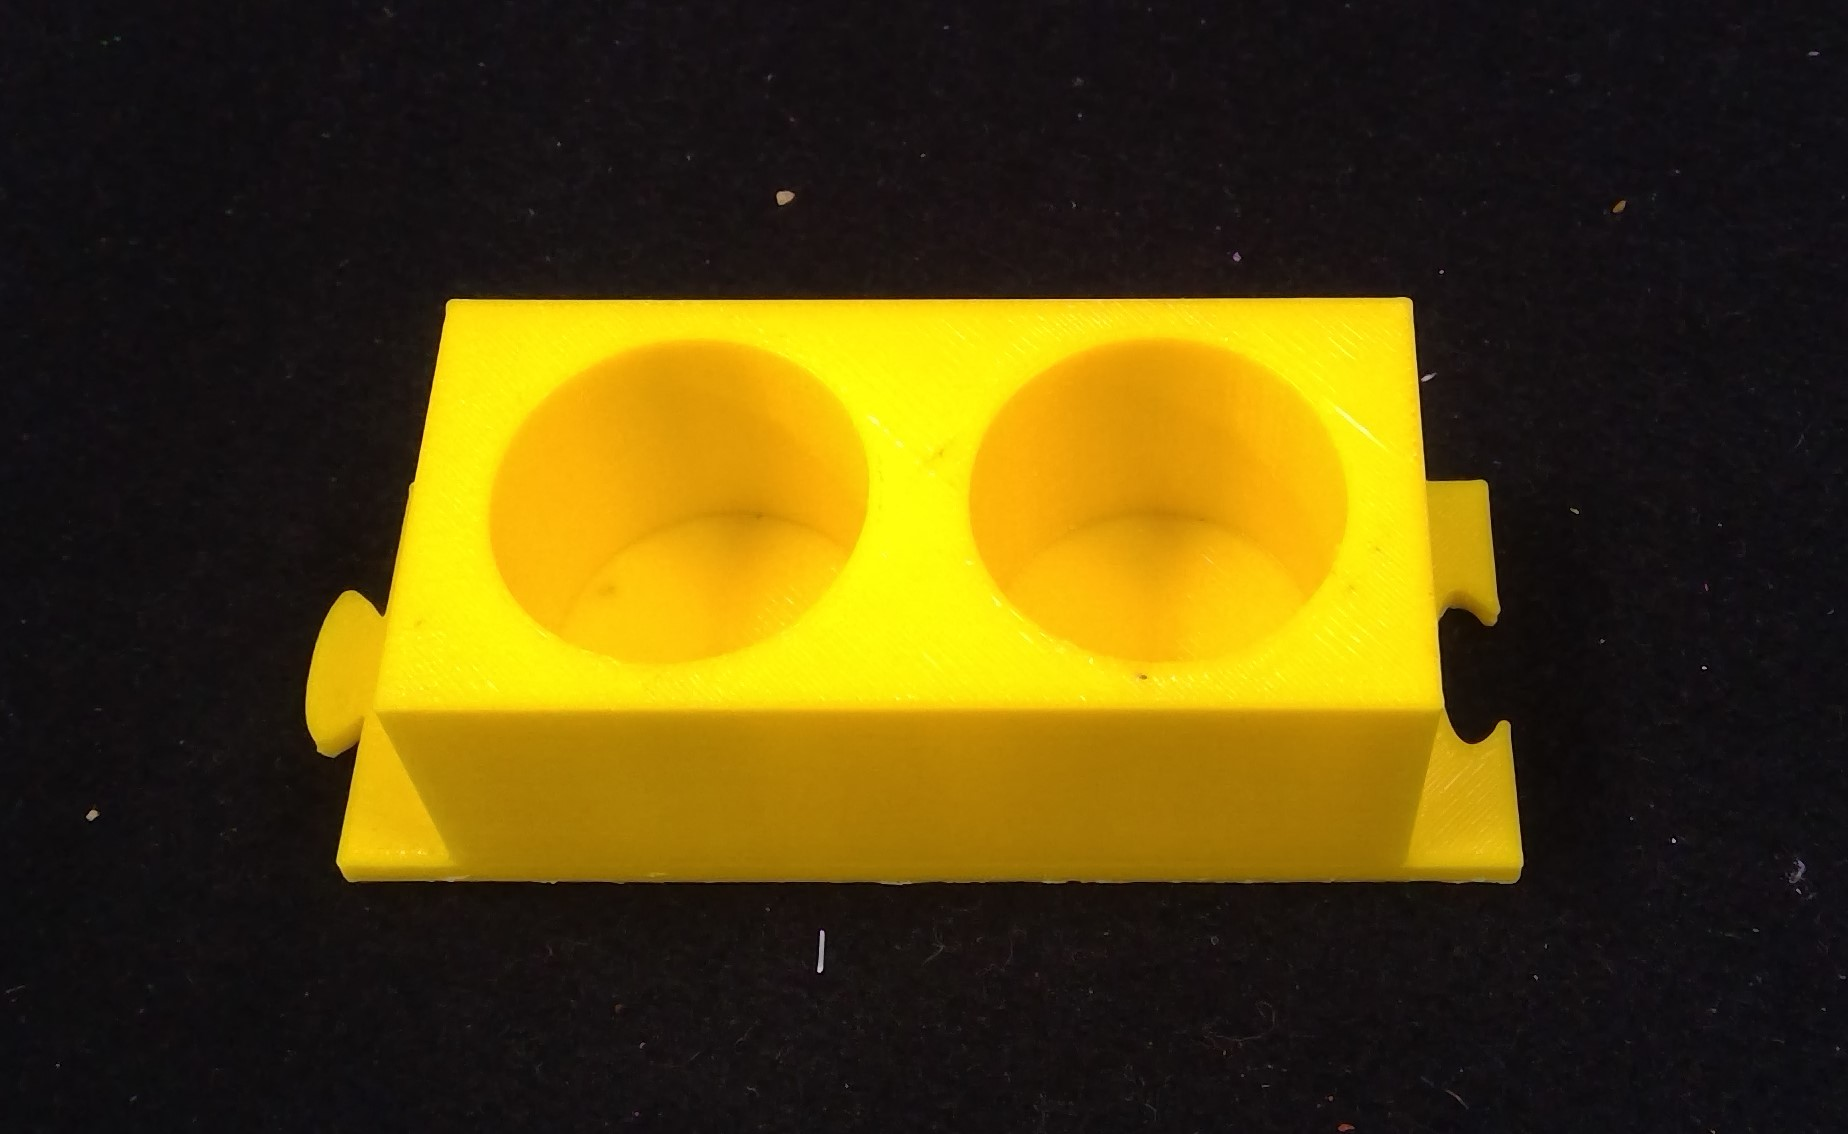
\includegraphics[width = 0.49\columnwidth]{bincase.jpg}
  %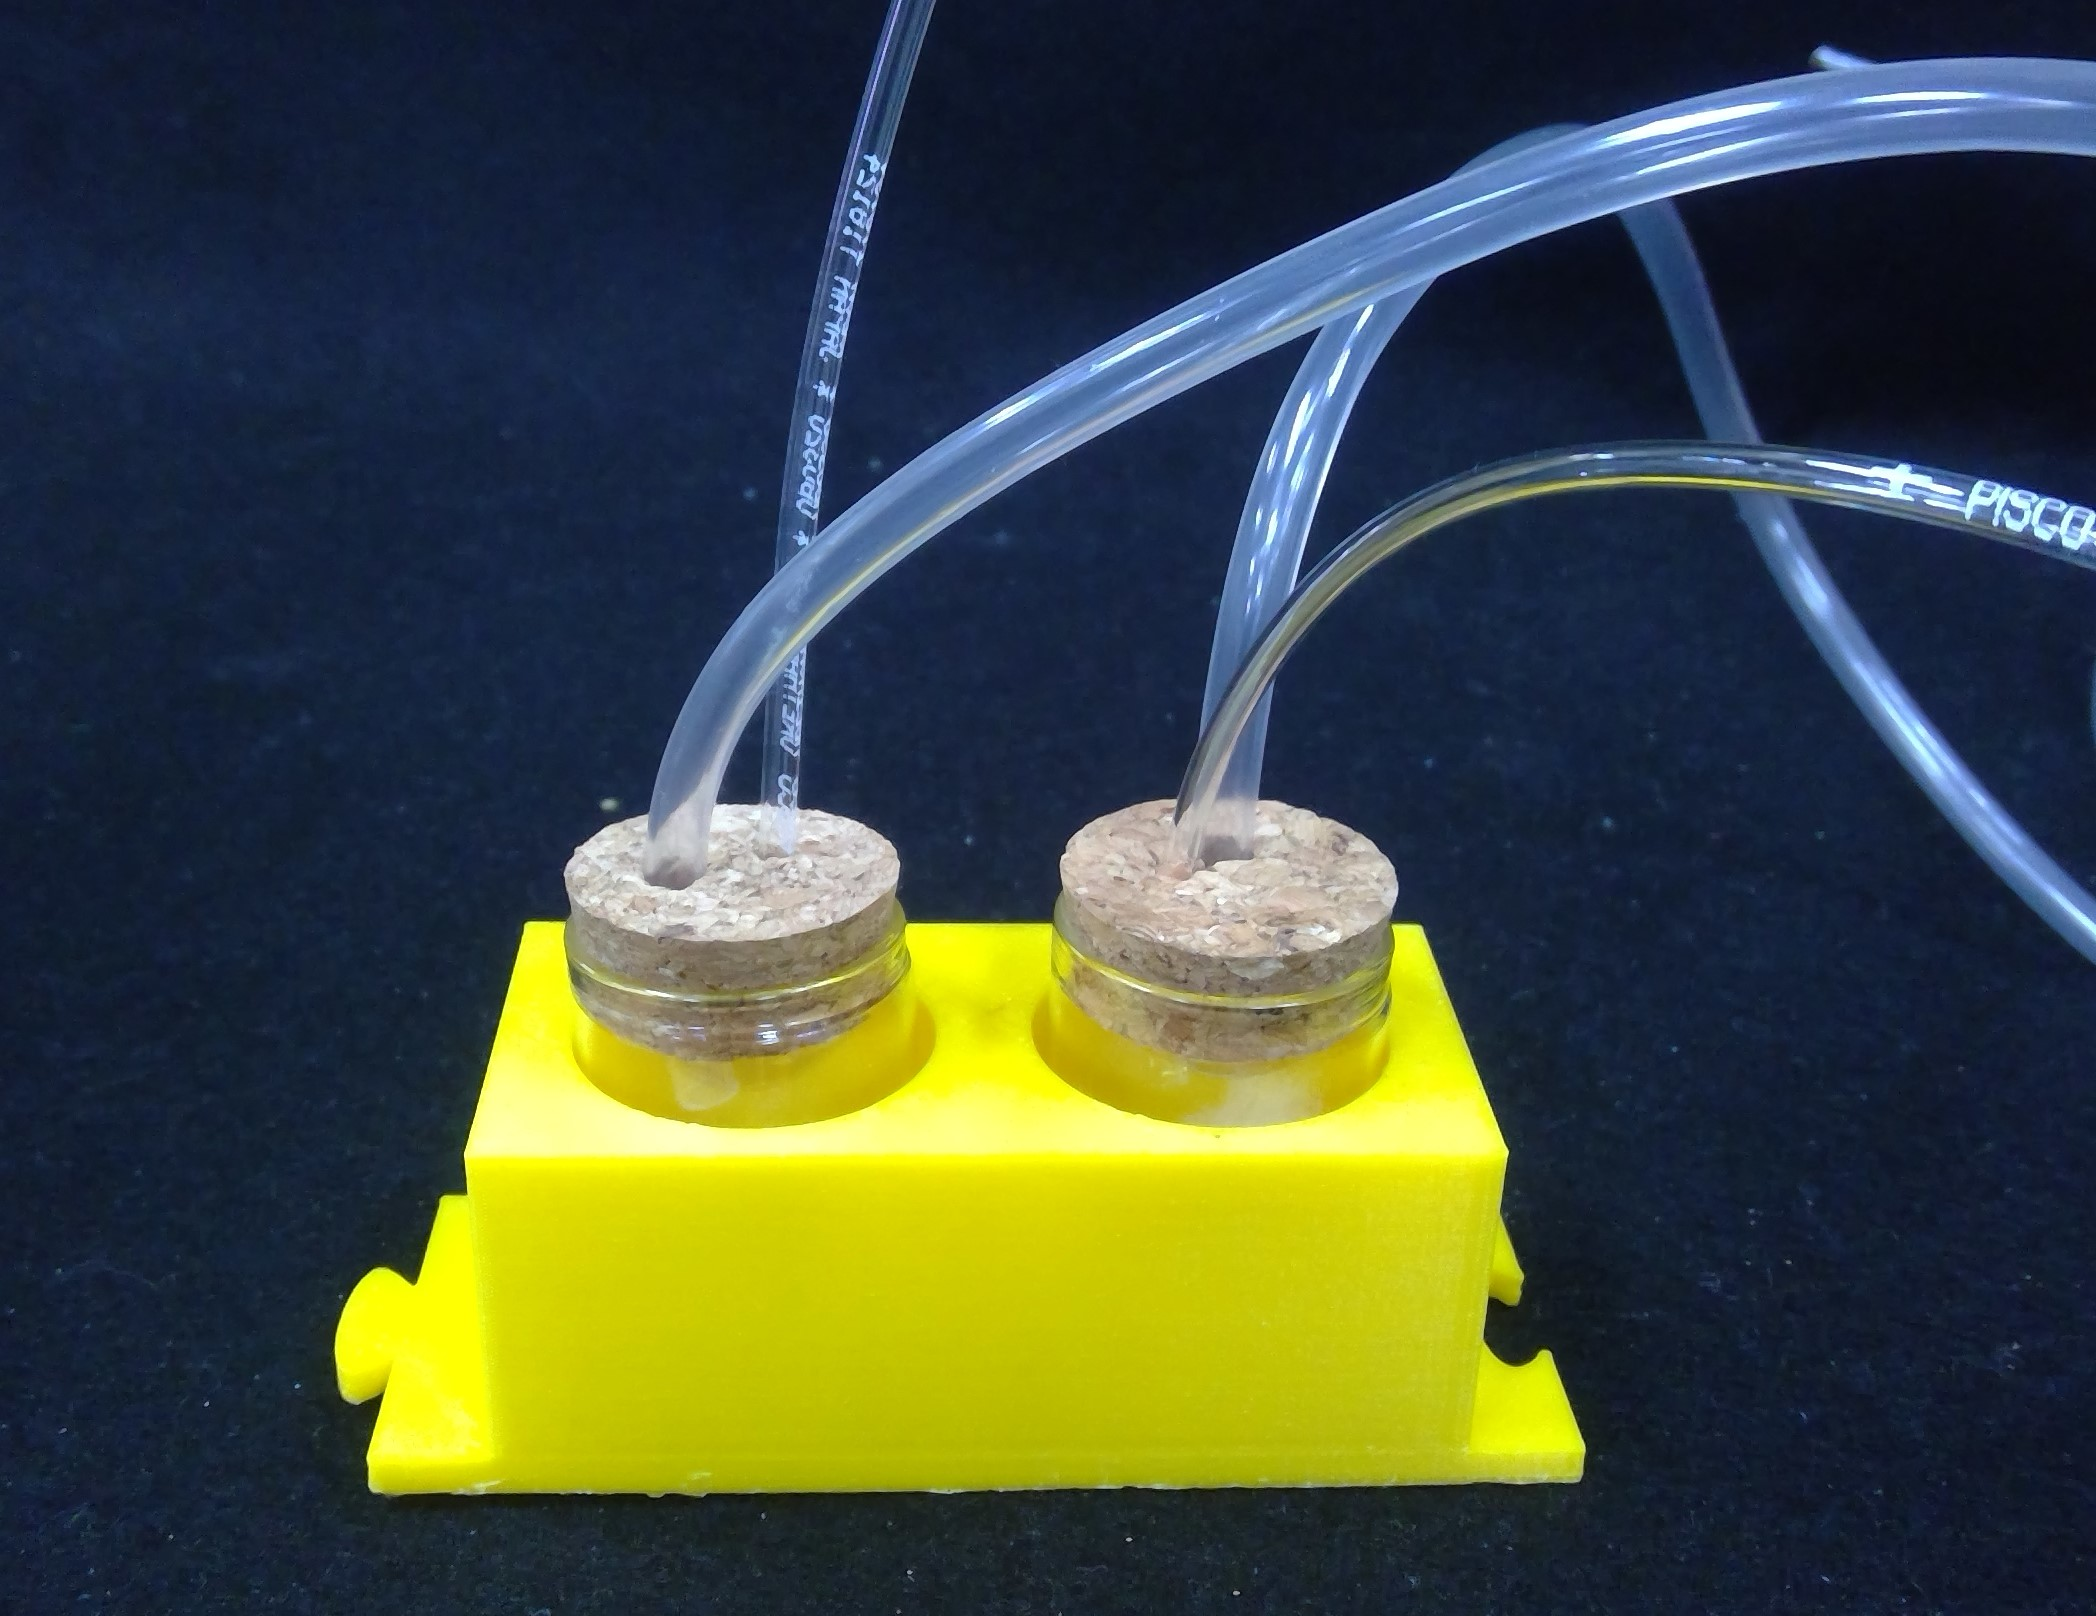
\includegraphics[scale = 0.075]{flavorcase.jpg}
  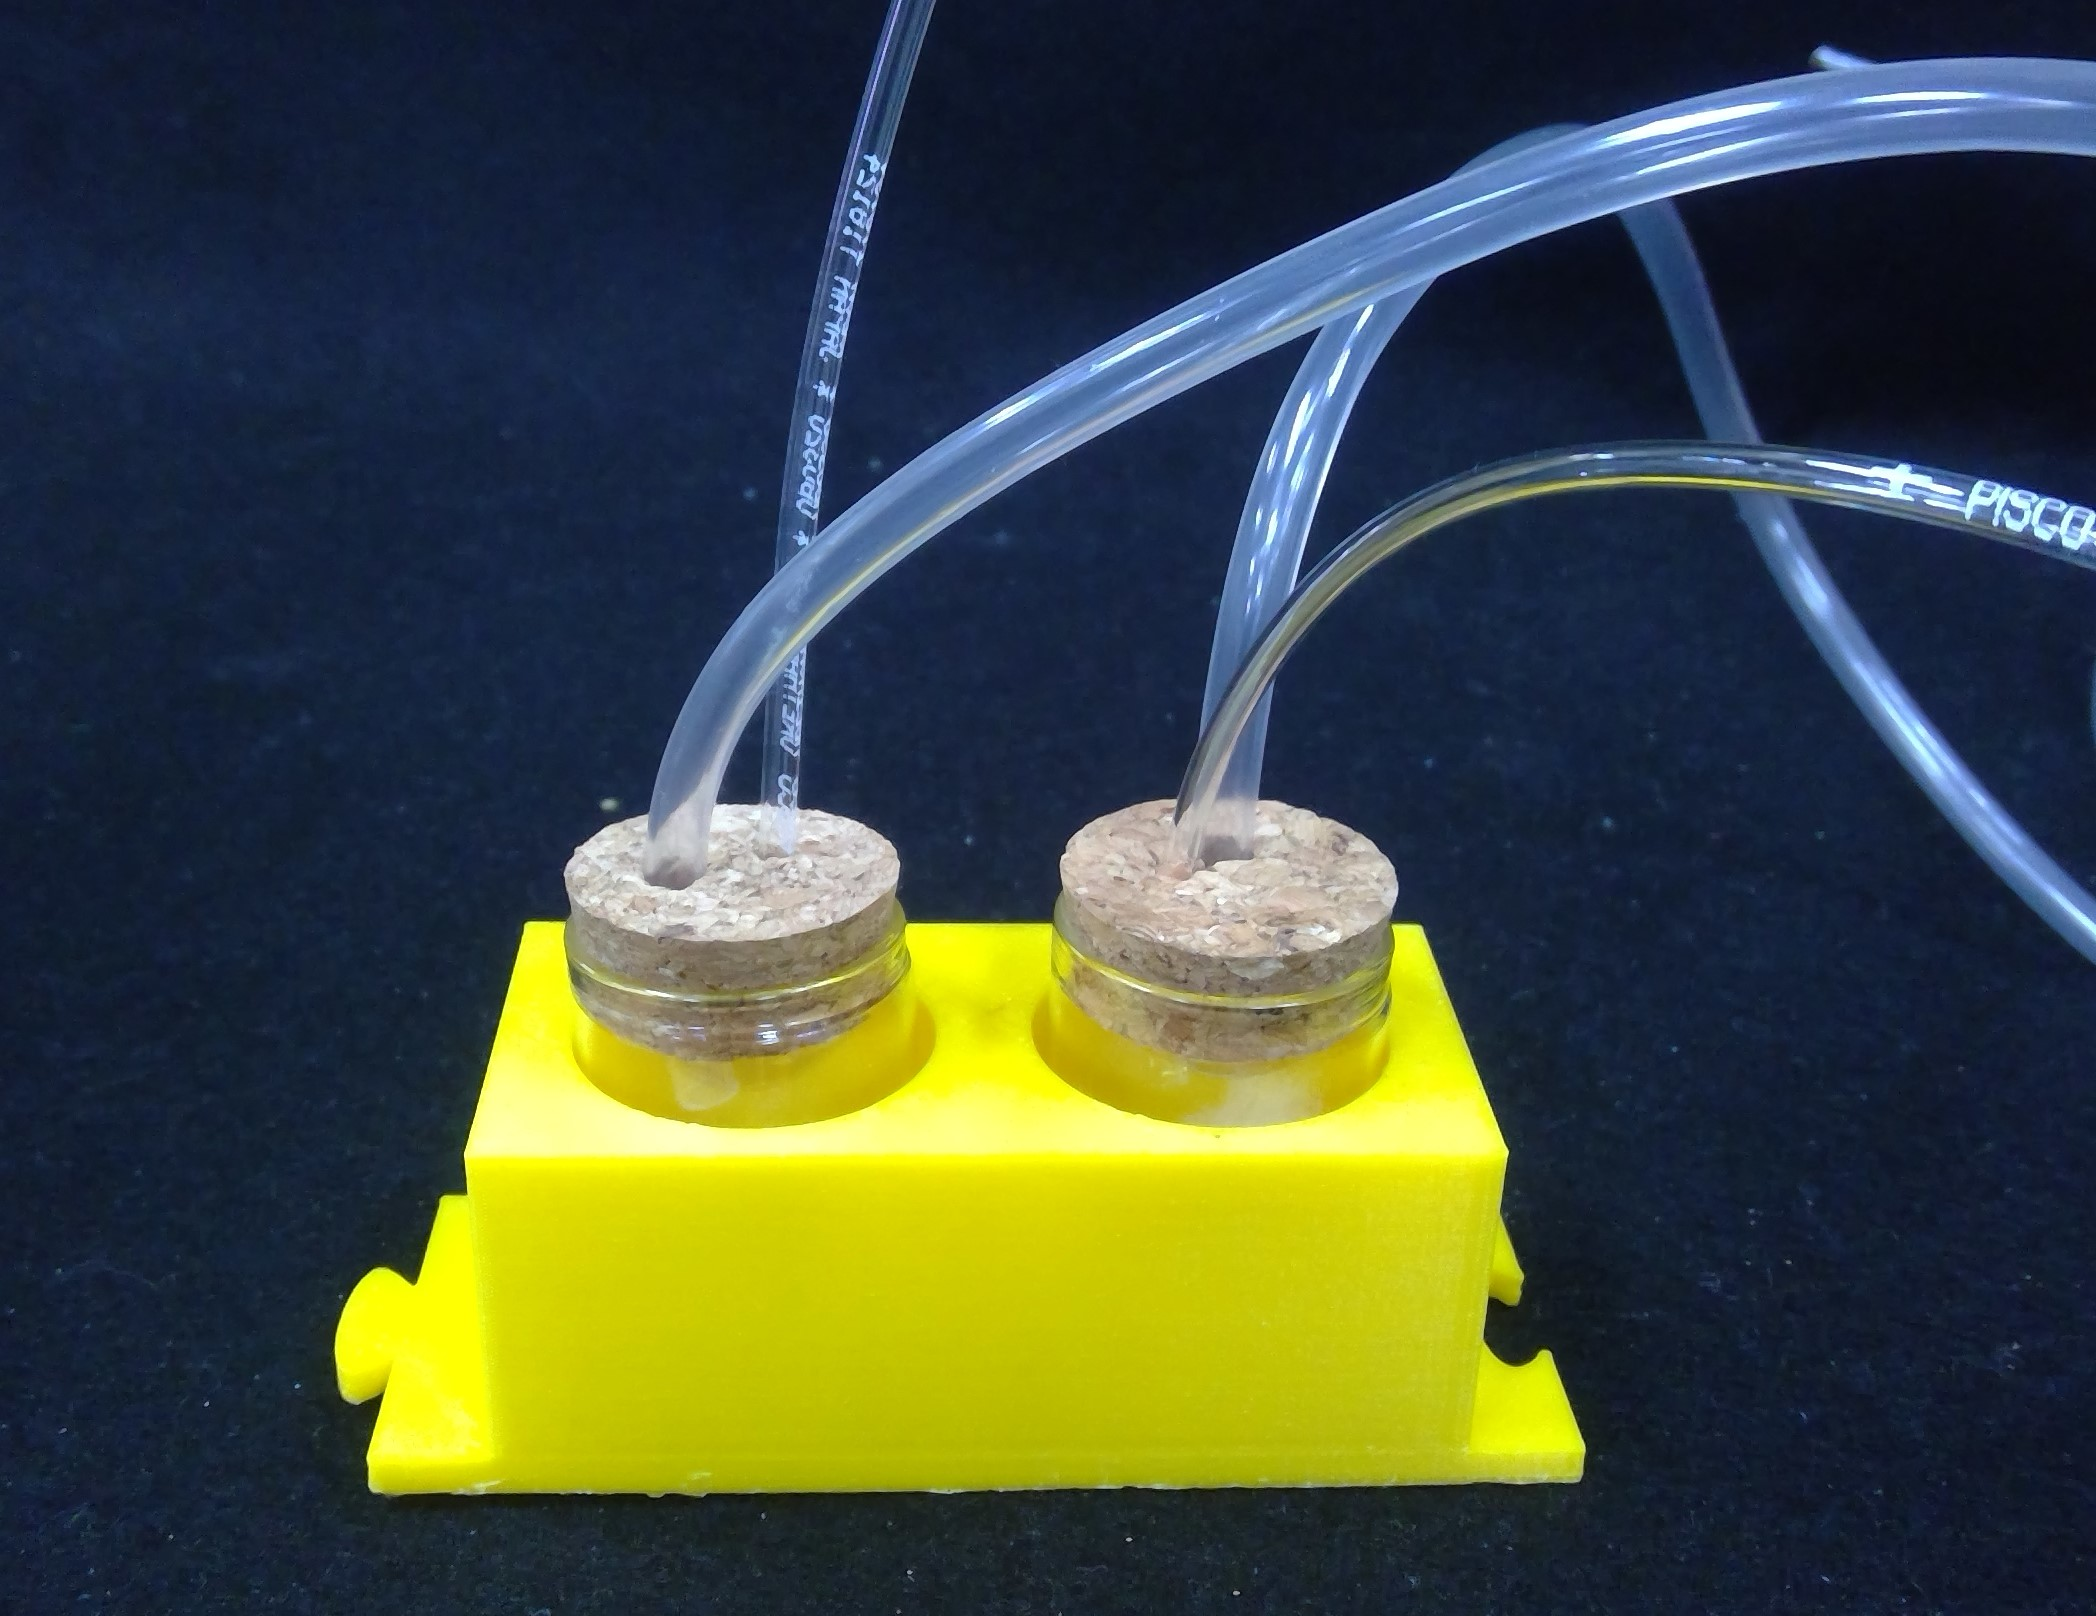
\includegraphics[width = 1.0\columnwidth]{flavorcase.jpg}
  \caption{香り瓶と香りボックス}
  \label{flavor}
\end{figure}


これらをまとめた嗅覚情報提示装置はリアルタイムのスムーズな香りの切り替えを可能とする.また,不必要な香りの漏洩を少なからず防ぎ,部屋に香りが充満することによる実験の弊害を多少なりとも防ぐことにつながる.
